
\documentclass{article} % For LaTeX2e
\usepackage{iclr2022_conference,times}

% Optional math commands from https://github.com/goodfeli/dlbook_notation.
%%%%% NEW MATH DEFINITIONS %%%%%

\usepackage{amsmath,amsfonts,bm}
\usepackage{dsfont}

% Mark sections of captions for referring to divisions of figures
\newcommand{\figleft}{{\em (Left)}}
\newcommand{\figcenter}{{\em (Center)}}
\newcommand{\figright}{{\em (Right)}}
\newcommand{\figtop}{{\em (Top)}}
\newcommand{\figbottom}{{\em (Bottom)}}
\newcommand{\captiona}{{\em (a)}}
\newcommand{\captionb}{{\em (b)}}
\newcommand{\captionc}{{\em (c)}}
\newcommand{\captiond}{{\em (d)}}

% Highlight a newly defined term
\DeclareOldFontCommand{\bf}{\normalfont\bfseries}{\mathbf}
\newcommand{\newterm}[1]{{\bf #1}}


% Figure reference, lower-case.
\def\figref#1{figure~\ref{#1}}
% Figure reference, capital. For start of sentence
\def\Figref#1{Figure~\ref{#1}}
\def\twofigref#1#2{figures \ref{#1} and \ref{#2}}
\def\quadfigref#1#2#3#4{figures \ref{#1}, \ref{#2}, \ref{#3} and \ref{#4}}
% Section reference, lower-case.
\def\secref#1{section~\ref{#1}}
% Section reference, capital.
\def\Secref#1{Section~\ref{#1}}
% Reference to two sections.
\def\twosecrefs#1#2{sections \ref{#1} and \ref{#2}}
% Reference to three sections.
\def\secrefs#1#2#3{sections \ref{#1}, \ref{#2} and \ref{#3}}
% Reference to an equation, lower-case.
\def\eqref#1{equation~\ref{#1}}
% Reference to an equation, upper case
\def\Eqref#1{Equation~\ref{#1}}
% A raw reference to an equation---avoid using if possible
\def\plaineqref#1{\ref{#1}}
% Reference to a chapter, lower-case.
\def\chapref#1{chapter~\ref{#1}}
% Reference to an equation, upper case.
\def\Chapref#1{Chapter~\ref{#1}}
% Reference to a range of chapters
\def\rangechapref#1#2{chapters\ref{#1}--\ref{#2}}
% Reference to an algorithm, lower-case.
\def\algref#1{algorithm~\ref{#1}}
% Reference to an algorithm, upper case.
\def\Algref#1{Algorithm~\ref{#1}}
\def\twoalgref#1#2{algorithms \ref{#1} and \ref{#2}}
\def\Twoalgref#1#2{Algorithms \ref{#1} and \ref{#2}}
% Reference to a part, lower case
\def\partref#1{part~\ref{#1}}
% Reference to a part, upper case
\def\Partref#1{Part~\ref{#1}}
\def\twopartref#1#2{parts \ref{#1} and \ref{#2}}

\def\ceil#1{\lceil #1 \rceil}
\def\floor#1{\lfloor #1 \rfloor}
\def\1{\bm{1}}
\newcommand{\train}{\mathcal{D}}
\newcommand{\valid}{\mathcal{D_{\mathrm{valid}}}}
\newcommand{\test}{\mathcal{D_{\mathrm{test}}}}

\def\eps{{\epsilon}}


% Random variables
\def\rtau{{\bm{\tau}}}
\def\rtaup{{\bm{\tau'}}}
\def\reta{{\bm{\eta}}}
\def\ra{{\bm{a}}}
\def\rb{{\bm{b}}}
\def\rc{{\bm{c}}}
\def\rd{{\bm{d}}}
\def\re{{\bm{e}}}
\def\rf{{\bm{f}}}
\def\rg{{\bm{g}}}
\def\rh{{\bm{h}}}
\def\ri{{\bm{i}}}
\def\rj{{\bm{j}}}
\def\rk{{\bm{k}}}
\def\rl{{\bm{l}}}
% rm is already a command, just don't name any random variables m
\def\rn{{\bm{n}}}
\def\ro{{\bm{o}}}
\def\rp{{\bm{p}}}
\def\rq{{\bm{q}}}
\def\rr{{\bm{r}}}
\def\rs{{\bm{s}}}
\def\rt{{\bm{t}}}
\def\ru{{\bm{u}}}
\def\rv{{\bm{v}}}
\def\rw{{\bm{w}}}
\def\rx{{\bm{x}}}
\def\ry{{\bm{y}}}
\def\rz{{\bm{z}}}

% Random vectors
\def\rvepsilon{{\mathbf{\epsilon}}}
\def\rvtheta{{\mathbf{\theta}}}
\def\rva{{\mathbf{a}}}
\def\rvb{{\mathbf{b}}}
\def\rvc{{\mathbf{c}}}
\def\rvd{{\mathbf{d}}}
\def\rve{{\mathbf{e}}}
\def\rvf{{\mathbf{f}}}
\def\rvg{{\mathbf{g}}}
\def\rvh{{\mathbf{h}}}
\def\rvu{{\mathbf{i}}}
\def\rvj{{\mathbf{j}}}
\def\rvk{{\mathbf{k}}}
\def\rvl{{\mathbf{l}}}
\def\rvm{{\mathbf{m}}}
\def\rvn{{\mathbf{n}}}
\def\rvo{{\mathbf{o}}}
\def\rvp{{\mathbf{p}}}
\def\rvq{{\mathbf{q}}}
\def\rvr{{\mathbf{r}}}
\def\rvs{{\mathbf{s}}}
\def\rvt{{\mathbf{t}}}
\def\rvu{{\mathbf{u}}}
\def\rvv{{\mathbf{v}}}
\def\rvw{{\mathbf{w}}}
\def\rvx{{\mathbf{x}}}
\def\rvy{{\mathbf{y}}}
\def\rvz{{\mathbf{z}}}

% Elements of random vectors
\def\erva{{\textnormal{a}}}
\def\ervb{{\textnormal{b}}}
\def\ervc{{\textnormal{c}}}
\def\ervd{{\textnormal{d}}}
\def\erve{{\textnormal{e}}}
\def\ervf{{\textnormal{f}}}
\def\ervg{{\textnormal{g}}}
\def\ervh{{\textnormal{h}}}
\def\ervi{{\textnormal{i}}}
\def\ervj{{\textnormal{j}}}
\def\ervk{{\textnormal{k}}}
\def\ervl{{\textnormal{l}}}
\def\ervm{{\textnormal{m}}}
\def\ervn{{\textnormal{n}}}
\def\ervo{{\textnormal{o}}}
\def\ervp{{\textnormal{p}}}
\def\ervq{{\textnormal{q}}}
\def\ervr{{\textnormal{r}}}
\def\ervs{{\textnormal{s}}}
\def\ervt{{\textnormal{t}}}
\def\ervu{{\textnormal{u}}}
\def\ervv{{\textnormal{v}}}
\def\ervw{{\textnormal{w}}}
\def\ervx{{\textnormal{x}}}
\def\ervy{{\textnormal{y}}}
\def\ervz{{\textnormal{z}}}

% Random matrices
\def\rmA{{\mathbf{A}}}
\def\rmB{{\mathbf{B}}}
\def\rmC{{\mathbf{C}}}
\def\rmD{{\mathbf{D}}}
\def\rmE{{\mathbf{E}}}
\def\rmF{{\mathbf{F}}}
\def\rmG{{\mathbf{G}}}
\def\rmH{{\mathbf{H}}}
\def\rmI{{\mathbf{I}}}
\def\rmJ{{\mathbf{J}}}
\def\rmK{{\mathbf{K}}}
\def\rmL{{\mathbf{L}}}
\def\rmM{{\mathbf{M}}}
\def\rmN{{\mathbf{N}}}
\def\rmO{{\mathbf{O}}}
\def\rmP{{\mathbf{P}}}
\def\rmQ{{\mathbf{Q}}}
\def\rmR{{\mathbf{R}}}
\def\rmS{{\mathbf{S}}}
\def\rmT{{\mathbf{T}}}
\def\rmU{{\mathbf{U}}}
\def\rmV{{\mathbf{V}}}
\def\rmW{{\mathbf{W}}}
\def\rmX{{\mathbf{X}}}
\def\rmY{{\mathbf{Y}}}
\def\rmZ{{\mathbf{Z}}}

% Elements of random matrices
\def\ermA{{\textnormal{A}}}
\def\ermB{{\textnormal{B}}}
\def\ermC{{\textnormal{C}}}
\def\ermD{{\textnormal{D}}}
\def\ermE{{\textnormal{E}}}
\def\ermF{{\textnormal{F}}}
\def\ermG{{\textnormal{G}}}
\def\ermH{{\textnormal{H}}}
\def\ermI{{\textnormal{I}}}
\def\ermJ{{\textnormal{J}}}
\def\ermK{{\textnormal{K}}}
\def\ermL{{\textnormal{L}}}
\def\ermM{{\textnormal{M}}}
\def\ermN{{\textnormal{N}}}
\def\ermO{{\textnormal{O}}}
\def\ermP{{\textnormal{P}}}
\def\ermQ{{\textnormal{Q}}}
\def\ermR{{\textnormal{R}}}
\def\ermS{{\textnormal{S}}}
\def\ermT{{\textnormal{T}}}
\def\ermU{{\textnormal{U}}}
\def\ermV{{\textnormal{V}}}
\def\ermW{{\textnormal{W}}}
\def\ermX{{\textnormal{X}}}
\def\ermY{{\textnormal{Y}}}
\def\ermZ{{\textnormal{Z}}}

% Vectors
\def\vzero{{\bm{0}}}
\def\vone{{\bm{1}}}
\def\vmu{{\bm{\mu}}}
\def\vthetap{\bm{\theta'}}
\def\vtheta{{\bm{\theta}}}
\def\vphi{{\bm{\phi}}}
\def\vphip{{\bm{\phi'}}}
\def\vpsi{{\bm{\psi}}}
\def\va{{\bm{a}}}
\def\vb{{\bm{b}}}
\def\vc{{\bm{c}}}
\def\vd{{\bm{d}}}
\def\ve{{\bm{e}}}
\def\vf{{\bm{f}}}
\def\vg{{\bm{g}}}
\def\vh{{\bm{h}}}
\def\vi{{\bm{i}}}
\def\vj{{\bm{j}}}
\def\vk{{\bm{k}}}
\def\vl{{\bm{l}}}
\def\vm{{\bm{m}}}
\def\vn{{\bm{n}}}
\def\vo{{\bm{o}}}
\def\vp{{\bm{p}}}
\def\vq{{\bm{q}}}
\def\vr{{\bm{r}}}
\def\vs{{\bm{s}}}
\def\vt{{\bm{t}}}
\def\vu{{\bm{u}}}
\def\vv{{\bm{v}}}
\def\vw{{\bm{w}}}
\def\vx{{\bm{x}}}
\def\vy{{\bm{y}}}
\def\vz{{\bm{z}}}

% Elements of vectors
\def\evalpha{{\alpha}}
\def\evbeta{{\beta}}
\def\evepsilon{{\epsilon}}
\def\evlambda{{\lambda}}
\def\evomega{{\omega}}
\def\evmu{{\mu}}
\def\evpsi{{\psi}}
\def\evsigma{{\sigma}}
\def\evtheta{{\theta}}
\def\eva{{a}}
\def\evb{{b}}
\def\evc{{c}}
\def\evd{{d}}
\def\eve{{e}}
\def\evf{{f}}
\def\evg{{g}}
\def\evh{{h}}
\def\evi{{i}}
\def\evj{{j}}
\def\evk{{k}}
\def\evl{{l}}
\def\evm{{m}}
\def\evn{{n}}
\def\evo{{o}}
\def\evp{{p}}
\def\evq{{q}}
\def\evr{{r}}
\def\evs{{s}}
\def\evt{{t}}
\def\evu{{u}}
\def\evv{{v}}
\def\evw{{w}}
\def\evx{{x}}
\def\evy{{y}}
\def\evz{{z}}

% Matrix
\def\mA{{\bm{A}}}
\def\mB{{\bm{B}}}
\def\mC{{\bm{C}}}
\def\mD{{\bm{D}}}
\def\mE{{\bm{E}}}
\def\mF{{\bm{F}}}
\def\mG{{\bm{G}}}
\def\mH{{\bm{H}}}
\def\mI{{\bm{I}}}
\def\mJ{{\bm{J}}}
\def\mK{{\bm{K}}}
\def\mL{{\bm{L}}}
\def\mM{{\bm{M}}}
\def\mN{{\bm{N}}}
\def\mO{{\bm{O}}}
\def\mP{{\bm{P}}}
\def\mQ{{\bm{Q}}}
\def\mR{{\bm{R}}}
\def\mS{{\bm{S}}}
\def\mT{{\bm{T}}}
\def\mU{{\bm{U}}}
\def\mV{{\bm{V}}}
\def\mW{{\bm{W}}}
\def\mX{{\bm{X}}}
\def\mY{{\bm{Y}}}
\def\mZ{{\bm{Z}}}
\def\mBeta{{\bm{\beta}}}
\def\mPhi{{\bm{\Phi}}}
\def\mLambda{{\bm{\Lambda}}}
\def\mSigma{{\bm{\Sigma}}}

% Tensor
\DeclareMathAlphabet{\mathsfit}{\encodingdefault}{\sfdefault}{m}{sl}
\SetMathAlphabet{\mathsfit}{bold}{\encodingdefault}{\sfdefault}{bx}{n}
\newcommand{\tens}[1]{\bm{\mathsfit{#1}}}
\def\tA{{\tens{A}}}
\def\tB{{\tens{B}}}
\def\tC{{\tens{C}}}
\def\tD{{\tens{D}}}
\def\tE{{\tens{E}}}
\def\tF{{\tens{F}}}
\def\tG{{\tens{G}}}
\def\tH{{\tens{H}}}
\def\tI{{\tens{I}}}
\def\tJ{{\tens{J}}}
\def\tK{{\tens{K}}}
\def\tL{{\tens{L}}}
\def\tM{{\tens{M}}}
\def\tN{{\tens{N}}}
\def\tO{{\tens{O}}}
\def\tP{{\tens{P}}}
\def\tQ{{\tens{Q}}}
\def\tR{{\tens{R}}}
\def\tS{{\tens{S}}}
\def\tT{{\tens{T}}}
\def\tU{{\tens{U}}}
\def\tV{{\tens{V}}}
\def\tW{{\tens{W}}}
\def\tX{{\tens{X}}}
\def\tY{{\tens{Y}}}
\def\tZ{{\tens{Z}}}


% Graph
\def\gA{{\mathcal{A}}}
\def\gB{{\mathcal{B}}}
\def\gC{{\mathcal{C}}}
\def\gD{{\mathcal{D}}}
\def\gE{{\mathcal{E}}}
\def\gF{{\mathcal{F}}}
\def\gG{{\mathcal{G}}}
\def\gH{{\mathcal{H}}}
\def\gI{{\mathcal{I}}}
\def\gJ{{\mathcal{J}}}
\def\gK{{\mathcal{K}}}
\def\gL{{\mathcal{L}}}
\def\gM{{\mathcal{M}}}
\def\gN{{\mathcal{N}}}
\def\gO{{\mathcal{O}}}
\def\gP{{\mathcal{P}}}
\def\gQ{{\mathcal{Q}}}
\def\gR{{\mathcal{R}}}
\def\gS{{\mathcal{S}}}
\def\gT{{\mathcal{T}}}
\def\gU{{\mathcal{U}}}
\def\gV{{\mathcal{V}}}
\def\gW{{\mathcal{W}}}
\def\gX{{\mathcal{X}}}
\def\gY{{\mathcal{Y}}}
\def\gZ{{\mathcal{Z}}}

% Sets
\def\sA{{\mathbb{A}}}
\def\sB{{\mathbb{B}}}
\def\sC{{\mathbb{C}}}
\def\sD{{\mathbb{D}}}
% Don't use a set called E, because this would be the same as our symbol
% for expectation.
\def\sF{{\mathbb{F}}}
\def\sG{{\mathbb{G}}}
\def\sH{{\mathbb{H}}}
\def\sI{{\mathbb{I}}}
\def\sJ{{\mathbb{J}}}
\def\sK{{\mathbb{K}}}
\def\sL{{\mathbb{L}}}
\def\sM{{\mathbb{M}}}
\def\sN{{\mathbb{N}}}
\def\sO{{\mathbb{O}}}
\def\sP{{\mathbb{P}}}
\def\sQ{{\mathbb{Q}}}
\def\sR{{\mathbb{R}}}
\def\sS{{\mathbb{S}}}
\def\sT{{\mathbb{T}}}
\def\sU{{\mathbb{U}}}
\def\sV{{\mathbb{V}}}
\def\sW{{\mathbb{W}}}
\def\sX{{\mathbb{X}}}
\def\sY{{\mathbb{Y}}}
\def\sZ{{\mathbb{Z}}}

% Entries of a matrix
\def\emLambda{{\Lambda}}
\def\emA{{A}}
\def\emB{{B}}
\def\emC{{C}}
\def\emD{{D}}
\def\emE{{E}}
\def\emF{{F}}
\def\emG{{G}}
\def\emH{{H}}
\def\emI{{I}}
\def\emJ{{J}}
\def\emK{{K}}
\def\emL{{L}}
\def\emM{{M}}
\def\emN{{N}}
\def\emO{{O}}
\def\emP{{P}}
\def\emQ{{Q}}
\def\emR{{R}}
\def\emS{{S}}
\def\emT{{T}}
\def\emU{{U}}
\def\emV{{V}}
\def\emW{{W}}
\def\emX{{X}}
\def\emY{{Y}}
\def\emZ{{Z}}
\def\emSigma{{\Sigma}}

% entries of a tensor
% Same font as tensor, without \bm wrapper
\newcommand{\etens}[1]{\mathsfit{#1}}
\def\etLambda{{\etens{\Lambda}}}
\def\etA{{\etens{A}}}
\def\etB{{\etens{B}}}
\def\etC{{\etens{C}}}
\def\etD{{\etens{D}}}
\def\etE{{\etens{E}}}
\def\etF{{\etens{F}}}
\def\etG{{\etens{G}}}
\def\etH{{\etens{H}}}
\def\etI{{\etens{I}}}
\def\etJ{{\etens{J}}}
\def\etK{{\etens{K}}}
\def\etL{{\etens{L}}}
\def\etM{{\etens{M}}}
\def\etN{{\etens{N}}}
\def\etO{{\etens{O}}}
\def\etP{{\etens{P}}}
\def\etQ{{\etens{Q}}}
\def\etR{{\etens{R}}}
\def\etS{{\etens{S}}}
\def\etT{{\etens{T}}}
\def\etU{{\etens{U}}}
\def\etV{{\etens{V}}}
\def\etW{{\etens{W}}}
\def\etX{{\etens{X}}}
\def\etY{{\etens{Y}}}
\def\etZ{{\etens{Z}}}

% The true underlying data generating distribution
\newcommand{\pdata}{p_{\rm{data}}}
% The empirical distribution defined by the training set
\newcommand{\ptrain}{\hat{p}_{\rm{data}}}
\newcommand{\Ptrain}{\hat{P}_{\rm{data}}}
% The model distribution
\newcommand{\pmodel}{p_{\rm{model}}}
\newcommand{\Pmodel}{P_{\rm{model}}}
\newcommand{\ptildemodel}{\tilde{p}_{\rm{model}}}
% Stochastic autoencoder distributions
\newcommand{\pencode}{p_{\rm{encoder}}}
\newcommand{\pdecode}{p_{\rm{decoder}}}
\newcommand{\precons}{p_{\rm{reconstruct}}}

\newcommand{\laplace}{\mathrm{Laplace}} % Laplace distribution

\newcommand{\E}{\mathbb{E}}
\newcommand{\Ls}{\mathcal{L}}
\newcommand{\R}{\mathbb{R}}
\newcommand{\emp}{\tilde{p}}
\newcommand{\lr}{\alpha}
\newcommand{\reg}{\lambda}
\newcommand{\rect}{\mathrm{rectifier}}
\newcommand{\softmax}{\mathrm{softmax}}
\newcommand{\sigmoid}{\sigma}
\newcommand{\softplus}{\zeta}
\newcommand{\KL}{D_{\mathrm{KL}}}
\newcommand{\Var}{\mathrm{Var}}
\newcommand{\standarderror}{\mathrm{SE}}
\newcommand{\Cov}{\mathrm{Cov}}
% Wolfram Mathworld says $L^2$ is for function spaces and $\ell^2$ is for vectors
% But then they seem to use $L^2$ for vectors throughout the site, and so does
% wikipedia.
\newcommand{\normlzero}{L^0}
\newcommand{\normlone}{L^1}
\newcommand{\normltwo}{L^2}
\newcommand{\normlp}{L^p}
\newcommand{\normmax}{L^\infty}

\newcommand{\parents}{Pa} % See usage in notation.tex. Chosen to match Daphne's book.

\DeclareMathOperator*{\argmax}{arg\,max}
\DeclareMathOperator*{\argmin}{arg\,min}

\DeclareMathOperator{\sign}{sign}
\DeclareMathOperator{\Tr}{Tr}
\let\ab\allowbreak


% MDP (from CCRIG or VAL)
\newcommand{\G}{\mathbf{G}}
\newcommand{\g}{\mathbf{g}}
\newcommand{\SF}{\mathbf{S}}
\newcommand{\stf}{\mathbf{s}}
\newcommand{\St}{\mathbf{S}}
\newcommand{\st}{\mathbf{s}}
\newcommand{\zt}{\mathbf{z}}
\newcommand{\gt}{\mathbf{g}}
\newcommand{\At}{\mathbf{A}}
\newcommand{\at}{\mathbf{a}}
\newcommand{\dyn}{\rho(\st_{t+1} \mid \st_t, \at_t)}


%%%%%%% Advantage weighted definitions
% \newcommand{\acronym}{{AWAC}}
% \newcommand{\pinew}{{\pi_i}}
% \newcommand{\piold}{{\pi_{i-1}}}
\newcommand{\pinew}{{\pi_{k+1}}}
\newcommand{\piold}{{\pi_\beta}}
% \newcommand{\pinew}{{\pi_\text{new}}}
% \newcommand{\piold}{{\pi_\text{old}}}
% \newcommand{\piold}{{\pi_\text{old}}}
\newcommand{\replaybuffer}{{\gR}}
\newcommand{\buffer}{\beta}
\newcommand{\lagrangeawr}{\lambda}
\newcommand{\projectpage}{\href{https://awacrl.github.io/}{\textit{awacrl.github.io}}}
\newcommand{\AWACMETHOD}{Advantage Weighted Actor Critic\xspace}
\newcommand{\DTV}{D_\mathrm{TV}}


%%%%%%% IQL
\def\ourname{IQL\xspace}
\def\ournamepref{implicit\xspace}
\def\Ournamepref{Implicit\xspace}




%%%%%%% SkewFit

% Sets
\newcommand{\FullSpaceDim}{n}
\newcommand{\FullSpace}{{\mathbb{R}^\FullSpaceDim}}
\newcommand{\Imgs}{{\mathcal{S}}}
\newcommand{\nImgs}{{\overline{\gS}}}
\newcommand{\Ss}{{\mathcal{S}}}
\newcommand{\As}{{\mathcal{A}}}
\newcommand{\Gs}{{\mathcal{G}}}
\newcommand{\ImgSets}{{\sA}}
\newcommand{\support}{{\text{support}}}
\newcommand{\Rnn}{{\sR^{n\times n}}}
\newcommand{\validq}{\mathcal{Q}}

%\newcommand\comment[1]{\textcolor{red}{#1}}
\newcommand\strike{\bgroup\markoverwith{\textcolor{red}{\rule[0.5ex]{2pt}{0.4pt}}}\ULon}
\definecolor{darkgreen}{RGB}{0,180,56}
\newcommand{\NEW}[1]{\textcolor{darkgreen}{#1}}
% \newcommand{\NEW}[1]{\textcolor{Green}{#1}}
% \newcommand{\strike}[1]{\vphantom{#1}}
% \newcommand{\NEW}[1]{#1}
\newcommand{\sampleN}{\stackrel{N}{\sim}}
\newcommand{\fcaption}[1]{\caption{{\footnotesize{#1}}}}


\newcommand{\uniform}[1]{\text{Uniform}[#1]}
\newcommand{\simple}{\text{na\"{\i}ve}}
\newcommand{\dent}{{d_\gH}}
\newcommand{\maxent}{\gH_\text{max}}
\newcommand{\limt}{\lim_{t \rightarrow \infty}}
\newcommand{\set}[1]{#1_\text{set}}

\newcommand{\pap}{{\theta}}
\newcommand{\papprox}{{p_\pap}}
\newcommand{\papproxt}{{p_{\pap_t}}}
\newcommand{\papproxtt}{{p_{\pap_{t+1}}}}
\newcommand{\pspg}{p(\SF \mid \pg)}
\newcommand{\pspgt}{p(\SF \mid \pgt)}
\newcommand{\pspgtt}{p(\SF \mid \pgtt)}
\newcommand{\z}{{\mathbf{z}}}
\newcommand{\wt}{{w_{t, \alpha}}}

\newcommand{\bx}{\mathbf{x}}
\mathchardef\mhyphen="2D

\newcommand{\MI}{I(\G, \SF)}
\newcommand{\HG}{\gH(\G)}
\newcommand{\HGS}{\gH(\G \mid \SF)}


\newcommand{\Loss}{\mathcal{L}}
\newcommand{\SFLoss}{\mathcal{L}^\text{SF}}
\newcommand{\Lossq}{\mathcal{L}_\text{SKEW}}
\newcommand{\Lossp}{\mathcal{L}_\text{FIT}}
\newcommand{\pstate}{{p^S_{\pgparam}}}
\newcommand{\pstatet}{{p^S_{\pgparam_t}}}
\newcommand{\pstatett}{{p^S_{\pgparam_{t+1}}}}

\newcommand{\U}{{U_\Imgs}}
\newcommand{\UA}{{U_\gA}}
\newcommand{\dynamics}{{p_\mathrm{dyn}}}
% Generative model
\newcommand{\pgparam}{{\phi}}
\newcommand{\pgparamt}{{\pgparam_t}}
\newcommand{\pgparamtt}{{\pgparam_{t+1}}}
\newcommand{\pg}{{q^G_{\pgparam}}}
\newcommand{\pgt}{{q^G_{\pgparam_t}}}
\newcommand{\pgtt}{{q^G_{\pgparam_{t+1}}}}
% Empirical distribution
\newcommand{\pes}[1]{{p_{\text{emp}_{#1}}}}
\newcommand{\pe}{\pstate}
\newcommand{\pet}{\pstatet}
\newcommand{\pett}{\pstatett}
% Weighted empirical distribution
\newcommand{\pwe}{\textcolor{red}{\bar {q}}}
% Skewed distribution
\newcommand{\pskewed}{{p_{\text{skewed}}}}
\newcommand{\pskewedt}{{p_{\text{skewed}_t}}}
\newcommand{\pskeweds}[1]{{p_{\text{skewed}_{#1}}}}
\newcommand{\pskewedtt}{{p_{\text{skewed}_{t+1}}}}
\newcommand{\pskewedn}{{p_{\text{skewed}_n}}}
\newcommand{\pskewednn}{{p_{\text{skewed}_{n+1}}}}
% For proof
\newcommand{\pt}{{p_\theta}}
\newcommand{\ptt}{{p_\theta^t}}
\newcommand{\htt}{{\gH_\theta^t}}
\newcommand{\replay}{\mathcal{R}}

%% Notation switches
\newcommand{\qe}{{\hat {q}}}
% Weighted empirical distribution
\newcommand{\qwe}{{\bar {q}}}

\newcommand{\inX}{{\G}}
\newcommand{\outX}{{\SF}}
\newcommand{\x}{x}

\newcommand{\NOTE}[1]{\textcolor{red}{(#1)}}
\newcommand{\TODO}[1]{\textcolor{red}{(TODO: #1)}}
\newcommand{\METHOD}{Skew-Fit\xspace}
\newcommand{\METHODmath}{\text{Skew-Fit}}
\newcommand{\METHODRIG}{Skew-Fit with RIG\xspace}
\newcommand{\CONTRACTIVE}{contractive\xspace}
\newcommand{\ESTABLE}{$\epsilon$-stable}
\newcommand{\dynop}{{\mathcal{F}_\mathrm{dyn}}}
\newcommand{\UB}{\mathcal{L}}
\newcommand{\error}{e}

% DAIB

\def\methodname {domain adversarial information bottleneck{}}
\def\methodabbrv {DAIB{}}

% IQL
\usepackage{mathtools}

\newcommand{\D}{\mathcal{D}}
\newcommand{\U}{\mathcal{U}}
\newcommand{\St}{\mathcal{S}}
\newcommand{\A}{\mathcal{A}}
\newcommand{\defeq}{\vcentcolon=}

\usepackage{siunitx}
\usepackage{hyperref}
\usepackage{url}
\usepackage{amsmath}
\usepackage{amssymb}
\usepackage{bbm}
\usepackage{cleveref}
\usepackage{bbm}
% \usepackage{comment}
\usepackage{xspace}
% \usepackage{subfigure}
\usepackage{subcaption}
\usepackage{algpseudocode}
\usepackage{algorithm}
\usepackage{wrapfig}
\usepackage{lipsum}
\usepackage{booktabs, multirow} % for borders and merged ranges
\usepackage{soul}% for underlines
\usepackage{float}
\usepackage[english]{babel}
\usepackage{amsthm}
\usepackage{tablefootnote}
\usepackage[flushleft]{threeparttable}

\newtheorem{theorem}{Theorem}
\newtheorem{lemma}[theorem]{Lemma}
\newcommand{\comment}[1]{}
\newtheorem{corollary}{Corollary}[theorem]


\newenvironment{sproof}{%
  \renewcommand{\proofname}{ Proof Sketch}\proof}{\endproof}


\Crefname{equation}{Eqn.}{Eqns.}
\Crefname{figure}{Fig.}{Figs.}
\Crefname{tabular}{Tab.}{Tabs.}

\def\ourname{IQL\xspace}

\def\ournamepref{implicit\xspace}

\def\Ournamepref{Implicit\xspace}

\title{Offline Reinforcement Learning \\ with \Ournamepref Q-Learning}

\author{Ilya Kostrikov, Ashvin Nair \& Sergey Levine \\
Department of Electrical Engineering and Computer Science \\
University of California, Berkeley \\
\texttt{\{kostrikov,anair17\}@berkeley.edu}, \texttt{svlevine@eecs.berkeley.edu} 
}

% The \author macro works with any number of authors. There are two commands
% used to separate the names and addresses of multiple authors: \And and \AND.
%
% Using \And between authors leaves it to \LaTeX{} to determine where to break
% the lines. Using \AND forces a linebreak at that point. So, if \LaTeX{}
% puts 3 of 4 authors names on the first line, and the last on the second
% line, try using \AND instead of \And before the third author name.

\newcommand{\fix}{\marginpar{FIX}}
\newcommand{\new}{\marginpar{NEW}}

\usepackage{mathtools}

\newcommand{\D}{\mathcal{D}}
\newcommand{\U}{\mathcal{U}}
\newcommand{\St}{\mathcal{S}}
\newcommand{\A}{\mathcal{A}}
\newcommand{\defeq}{\vcentcolon=}

\newcommand*{\DRAFT}{}  %
\newcommand{\ilya}[1]{\ifdefined\DRAFT \todo[inline,color=green!20!white]{\textbf{Ilya:} #1} \else \fi}
\newcommand{\ofir}[1]{\ifdefined\DRAFT \todo[inline,color=red!20!white]{\textbf{Ofir:} #1}  \else \fi}
\newcommand{\ofirc}[1]{\ifdefined\DRAFT \textcolor{magenta}{red: #1} \else \fi}

\newcommand{\jonathan}[1]{\ifdefined\DRAFT \todo[inline,color=magenta!20!white]{\textbf{Jonathan:} #1} \else \fi}
\newcommand{\jonathanc}[1]{\ifdefined\DRAFT \textcolor{magenta}{Jonathan: #1} \else \fi}

\newcommand{\rob}[1]{\ifdefined\DRAFT \todo[inline,color=cyan!20!white]{\textbf{Rob:} #1} \else \fi}
\newcommand{\robc}[1]{\ifdefined\DRAFT \textcolor{cyan}{Rob: #1} \else \fi}


\iclrfinalcopy % Uncomment for camera-ready version, but NOT for submission.
\begin{document}

\maketitle

\begin{abstract}
Offline reinforcement learning requires reconciling two conflicting aims: learning a policy that improves over the behavior policy that collected the dataset, while at the same time minimizing the deviation from the behavior policy so as to avoid errors due to distributional shift. This trade-off is critical, because most current offline reinforcement learning methods need to query the value of unseen actions during training to improve the policy, and therefore need to either constrain these actions to be in-distribution, or else regularize their values. We propose a new offline RL method that never needs to evaluate actions outside of the dataset, but still enables the learned policy to improve substantially over the best behavior in the data through generalization.
The main insight in our work is that, instead of evaluating unseen actions from the latest policy, we can approximate the policy improvement step implicitly by treating the state value function as a random variable, with randomness determined by the action (while still integrating over the dynamics to avoid excessive optimism), and then taking a state conditional upper expectile of this random variable to estimate the value of the best actions in that state. This leverages the generalization capacity of the function approximator to estimate the value of the best available action at a given state without ever directly querying a Q-function with this unseen action.
Our algorithm alternates between fitting this upper expectile value function and backing it up into a Q-function, without any explicit policy. Then, we extract the policy via advantage-weighted behavioral cloning, which also avoids querying out-of-sample actions. We dub our method \ournamepref Q-learning (\ourname).  \ourname is easy to implement, computationally efficient, and only requires fitting an additional critic with an asymmetric L2 loss.
% \footnote{Our implementation is available at \href{https://github.com/ikostrikov/implicit\_policy\_improvement}{https://github.com/ikostrikov/implicit\_q\_learning}}
\ourname demonstrates the state-of-the-art performance on D4RL, a standard benchmark for offline reinforcement learning.
We also demonstrate that \ourname achieves strong performance fine-tuning using online interaction after offline initialization.
\end{abstract}

\section{Introduction}

% Reinforcement learning is a field of machine learning research that involves obtaining optimal policies from interactions with a learning environment. Off-policy reinforcement learning algorithms usually work with growing datasets collected by interactions with the environment with a learned policy. Nonetheless, these interactions with the learning environment are undesirable in various real-world applications since exploration can be expensive and unsafe. At the same time, standards methods for off-policy reinforcement learning assume complete action coverage and are not capable of learning on datasets with sparse action coverage that commonly occur in real-world problems.
% Finally, offline (batch) reinforcement learning studies algorithms that are capable of learning from fixed datasets without additional exploration~\citep{fujimoto2019off, lange2012batch}. Due to the lack of exploration, one of the main challenges associated with offline reinforcement learning is constraining policy optimization to an available static dataset. While previous methods address this problem by introducing soft constraints that encourage training policy to stay close to the dataset, we introduce the first method that relies strictly on dataset transitions to obtain the optimal policy without sampling any actions throughout training.

%%SL.9.28: Here is a potential rephrasing here that I think could be more concise and to the point:
Offline reinforcement learning (RL) addresses the problem of learning effective policies entirely from previously collected data, without online interaction~\citep{fujimoto2019off, lange2012batch}. This is very appealing in a range of real-world domains, from robotics to logistics and operations research, where real-world exploration with untrained policies is costly or dangerous, but prior data is available. However, this also carries with it major challenges: improving the policy beyond the level of the behavior policy that collected the data requires estimating values for actions other than those that were seen in the dataset, and this, in turn, requires trading off policy improvement against distributional shift, since the values of actions that are too different from those in the data are unlikely to be estimated accurately. Prior methods generally address this by either constraining the policy to limit how far it deviates from the behavior policy~\citep{fujimoto2019off, wu2019behavior, fujimoto2021minimalist, kumar2019stabilizing, nair2020awac, wang2020critic}, or by regularizing the learned value functions to assign low values to out-of-distribution actions~\citep{kumar2020conservative, kostrikov2021offline}. Nevertheless, this imposes a trade-off between how much the policy improves and how vulnerable it is to misestimation due to distributional shift. Can we devise an offline RL method that avoids this issue by never needing to directly query or estimate values for actions that were not seen in the data?
%%SL.9.28: This then sets the stage for us to present our idea next, without quite so much of a drawn out discussion.

% Prior work on offline reinforcement learning builds on temporal difference (TD) learning.
% However, TD learning involves learning policy values based on estimates for the future state using actions sampled from the current policy, defined when supported by the dataset.
%%SL.9.21: Above sentence is pretty hard for me to parse, consider rewriting -- I think you mean something like:
% However, using TD learning to learn the optimal value function requires estimating the value of the current policy, which is typically done by querying a Q-function with actions from the current policy. In the offline setting, these actions are usually \emph{out-of-distribution} relative to the data distribution on which this Q-function is trained, which comes from the behavior policy.
% Thus, the recent methods focus on regularizing the learned policies or critics to stay close to the datasets.
%%SL.9.13: I don't think we should say that -- offline RL and batch RL goes way further back, and this is not even the first deep offline RL method (I don't know which one was first, but at least QT-Opt did offline RL in mid-2018, and it wouldn't surprise me if there were others prior to that)
% For example, prior methods constrain the action selection to the dataset action distribution via a density model~\citep{fujimoto2019off}, applying explicit~\citep{wu2019behavior, fujimoto2021minimalist, kumar2019stabilizing} or implicit~\citep{nair2020awac, wang2020critic} divergence constraints to the learned policy, or by directly regularizing the critic to avoid high values for out-of-distribution actions~\citep{kumar2020conservative, kostrikov2021offline}. However, these methods only mitigate the issue and do not prevent querying values of out-of-distribution actions altogether.
%%SL.9.21: it might not be 100% obvious to the reader why this is true -- could clarify that there is always a fundamental tension, since we want the learned policy to deviate from the behavior policy, but not so much that it results in high errors [or something like that]
% At the same time, one cannot have any guarantees regarding these values, which can cripple learning since in the tabular case, these values are not defined, while in the function approximation case, we cannot guarantee generalization since the actions might not only be outside the dataset but also \emph{out-of-distribution}.
%%SL.9.13: This paragraph would read better if we more clearly motivate the individual decisions before presenting them. Perhaps one way to do this is to first briefly motivate why querying unseen actions is risky, then pose the question: If we do not query a Q-function with actions other than those that were taken in the dataset, how can we determine that it's possible for a learned policy to do better than the dataset action? We can then say that we leverage the fact that neural nets generalize across different states to train value functions with a quantile regression objective, effectively capturing an upper quantile of possible values that could be achieved from a given state
%%SL.9.28: If you go with my suggestion for para 1, I think para 2 can mostly be cut and/or folded into para 1. That way, para 1 lays out "what is the problem" "why is it hard" "why has prior work not solved it", and right in the second paragraph you can dive into motivating your method.

In this work, we start from an observation that \emph{in-distribution} constraints widely used in prior work might not be sufficient to avoid value function extrapolation, and we ask whether it is possible to learn an optimal policy with \emph{in-sample learning}, without \emph{ever} querying the values of any unseen actions.
% This work proposes an alternative approach to learning the optimal values constrained to a fixed dataset. 
The key idea in our method is to approximate an upper expectile of the distribution over values with respect to the distribution of dataset actions for each state. We alternate between fitting this value function with expectile regression, and then using it to compute Bellman backups for training the $Q$-function.
%%SL.10.3: 
We show that we can do this simply by modifying the loss function in a SARSA-style TD backup, without ever using out-of-sample actions in the target value.
Once this $Q$-function has converged, we extract the corresponding policy using advantage-weighted behavioral cloning.
%%SL.10.3: and then can comment out the sentence below (since this info is already above if you use my suggestion)
% Thus, our approach never queries $Q$ values for unseen actions, either to compute the Bellman backups or to extract the policy.
%%SL.9.28: Maybe add something like: 
This approach does not require explicit constraints or explicit regularization of out-of-distribution actions during value function training, though our policy extraction step does implicitly enforce a constraint, as discussed in prior work on advantage-weighted regression~\citep{peters2007reinforcement, peng2019advantage, nair2020awac, wang2020critic}.
%%AVN.10.4 Reordered chronologically
%%SL.9.28: Consider putting everything below this line into a separate paragraph that summarizes the contribution. I know it can be a bit redundant, but this is important to ensure that reviewers don't miss what is new. E.g., something like this: 

Our main contribution is \ournamepref Q-learning (\ourname), a new offline RL algorithm that avoids ever querying values of unseen actions while still being able to perform multi-step dynamic programming updates.
Our method is easy to implement by making a small change to the loss function in a simple SARSA-like TD update and is computationally very efficient. Furthermore, our approach demonstrates the state-of-the-art performance on D4RL, a popular benchmark for offline reinforcement learning. In particular, our approach significantly improves over the prior state-of-the-art on challenging Ant Maze tasks that require to ``stitch'' several sub-optimal trajectories. Finally, we demonstrate that our approach is suitable for finetuning; after initialization from offline RL, \ourname is capable of improving policy performance utilizing additional interactions.
%%SL.9.28: I wonder if it might help to go into more detail about the specific improvement in performance? Otherwise this sounds a little generic.
%% Ilya: Done.

\vspace{-0.1cm}
\section{Related work}
\vspace{-0.1cm}

A significant portion of recently proposed offline RL methods are based on either constrained or regularized approximate dynamic programming (e.g., Q-learning or actor-critic methods), with the constraint or regularizer serving to limit deviation from the behavior policy. We will refer to these methods as ``multi-step dynamic programming'' algorithms, since they perform true dynamic programming for multiple iterations, and therefore can in principle recover the optimal policy if provided with high-coverage data.
The constraints can be implemented via an explicit density model~\citep{wu2019behavior, fujimoto2019off, kumar2019stabilizing, ghasemipour2021emaq}, implicit divergence constraints~\citep{nair2020awac, wang2020critic, peters2007reinforcement, peng2019advantage, siegel2020keep}, or by adding a supervised learning term to the policy improvement objective~\citep{fujimoto2021minimalist}. Several works have also proposed to directly regularize the Q-function to produce low values for out-of-distribution actions~\citep{kostrikov2021offline, kumar2020conservative,fakoor2021continuous}. Our method is also a multi-step dynamic programming algorithm. However, in contrast to prior works, our method completely avoids directly querying the learned Q-function with unseen actions during training, removing the need for any constraint during this stage, though the subsequent policy extraction, which is based on advantage-weighted regression~\citep{peng2019advantage,nair2020awac}, does apply an implicit constraint. However, this policy does not actually influence value function training.

% A number of methods achieve impressive empirical results without dynamical programming. \cite{brandfonbrener2021offline} (Onestep RL) demonstrate a competitive performance of imitation learning algorithms on a variety of offline RL tasks. While \cite{chen2021decision} argues for imitation learning with an autoregressive sequential model. Although these methods are simple to implement and effective on the MuJoCo locomotion tasks in D4RL, we show that such imitation learning approaches generally do not perform well on more complex datasets that require combining parts of suboptimal trajectories (``stitching''). In contrast, methods based on approximate dynamic programming handle these cases much more effectively. We discuss this distinction in more detail in \cref{sec:example}. Our method maintains the simplicity of imitation learning methods but is capable of performing dynamical programming on the other hand.

In contrast to multi-step dynamic programming methods, several recent works have proposed methods that rely either on a single step of policy iteration, fitting the value function or Q-function of the behavior policy and then extracting the corresponding greedy policy~\citep{peng2019advantage,brandfonbrener2021offline,gulcehre2021regularized}, or else avoid value functions completely and utilize behavioral cloning-style objectives~\citep{chen2021decision}. We collectively refer to these as ``single-step''
%%SL.10.3: We can use any name you want, but we must be consistent about it. In experiments, you sometimes refer to them as single-step policy evaluation or something like that, that's fine too, but we should make sure we use exactly the same term throughout.
approaches. These methods avoid needing to query unseen actions as well, since they either use no value function at all, or learn the value function of the behavior policy. Although these methods are simple to implement and effective on the MuJoCo locomotion tasks in D4RL, we show that such single-step methods perform very poorly on more complex datasets in D4RL, which require combining parts of suboptimal trajectories (``stitching''). Prior multi-step dynamic programming methods perform much better in such settings, as does our method. We discuss this distinction in more detail in \Cref{sec:example}. Our method also shares the simplicity and computational efficiency of single-step approaches, providing an appealing combination of the strengths of both types of methods.

Our method is based on estimating the characteristics of a random variable. Several recent works involve approximating statistical quantities of the value function distribution. In particular, quantile regression~\citep{koenker2001quantile} has been previously used in reinforcement learning to estimate the quantile function of a state-action value function~\citep{dabney2018distributional, dabney2018implicit,kuznetsov2020controlling}.
Although our method is related, in that we perform expectile regression, our aim is not to estimate the distribution of values that results from stochastic transitions, but rather estimate expectiles of the state value function with respect to random actions.
%%SL.9.28: are you sure you don't mean to say "state value function with respect to variability in the action"? that is, the action is the source of randomness
%%Ilya: I see why this sentence is confusing. Thinking how to paraphrase it.
%%SL.10.3: I rephrased it a bit
This is a very different statistic: our aim is not to determine how the $Q$-value can vary with different future outcomes, but how the $Q$-value can vary with different actions \emph{while averaging together future outcomes due to stochastic dynamics}. While prior work on distributional RL can also be used for offline RL, it would suffer from the same action extrapolation issues as other methods, and would require similar constraints or regularization, while our method does not.

%%SL.9.28: I think you can probably just cut this paragraph, and cover all these papers in preceding paragraphs. Otherwise, I think this might just get too much. The main thrust of related work should really be around (1) multi-step; (2) single-step; (3) resolve confusion wrt distributional
% After training the value function, our method must extract a policy from the value function when learning in continuous action spaces. To avoid the need to query unseen actions during policy extraction, we employ a widely used weighted behavioral cloning~\citep{peters2007reinforcement, nair2020awac, wang2020critic, peng2019advantage, siegel2020keep}. However, we do not use samples from the current learning policy to estimate the advantage in contrast to these methods.


\section{Preliminaries}

The RL problem is formulated in the context of a Markov decision process (MDP) $(\St, \A, p_0(s), p(s'|s,a), r(s,a), \gamma)$, where $\St$ is a state space, $\A$ is an action space, $p_0(s)$ is a distribution of initial states, $p(s' | s, a)$ is the environment dynamics, $r(s,a)$ is a reward function, and $\gamma$ is a discount factor. The agent interacts with the MDP according to a policy $\pi(a|s)$. The goal is to obtain a policy that maximizes the cumulative discounted returns: 
\vspace{-0.2cm}
$$\pi^* = \argmax_\pi \E_\pi\left[\sum_{t=0}^\infty\gamma^t r(s_t, a_t) | \allowbreak s_0 \sim p_0(\cdot), \allowbreak  a_t \sim \pi(\cdot|s_t), \allowbreak s_{t+1} \sim p(\cdot|s_t, a_t) \right].$$
%%SL.9.21: Maybe to make this equation a bit less imposing, you could just drop the stuff to the right of the conditioning bar in the expectation
Off-policy RL methods based on approximate dynamic programming typically utilize a state-action value function ($Q$-function), referred to as $Q(s, a)$, which corresponds to the discounted returns obtained by starting from the state $s$ and action $a$, and then following the policy $\pi$.
%%SL.10.3: Commenting out the sentence below for space and b/c we are not talking about our method yet
%We make no assumptions regarding the state and action spaces, and the proposed algorithms can be applied to discrete and continuous action spaces without significant modification.
\vspace{-0.3cm}
\paragraph{Offline reinforcement learning.} In contrast to online (on-policy or off-policy) RL methods, offline RL uses previously collected data without any additional data collection. Like many recent offline RL methods, our work builds on approximate dynamic programming methods that minimize temporal difference error, according to the following loss:
%%SL.9.28: I'm resisting calling these "actor-critic" to avoid confusion, since our value learning is *not* actor critic. I wonder also if it might be better to bite the bullet and just stick a "max" in the target value, and just avoid the policy all together. Our method doesn't use a policy until the end (extraction), and I feel like a lot of these concepts are much clearer when we present them as Q-learning rather than actor critic. As is, we don't actually explain how the actor is updated at all, which makes it non-obvious to the reader why overestimation would even happen. Another thing you could do, which I think will make Section 4 easier to understand, is introduce all the TD losses in the backup with a value function V(s') and then in the text say usually we take V(s') = Q(s',a') for SARSA, V(s') = E_{a' \sim \pi_\psi(a'|s')}[Q(s',a')] for actor-critic methods, and V(s') = max_{a'} Q(s',a') for Q-learning. Then it will be very natural in Section 4 to introduce your alternative way of estimating V(s'), while everything else stays unchanged.
\vspace{-0.1cm}
\begin{equation}
L_{TD}(\theta) = \E_{(s, a, s')\sim\D}[(r(s,a) + \gamma \max_{a'}Q_{\hat{\theta}}(s',a') - Q_\theta(s,a))^2],
\label{eqn:td}
\vspace{-0.2cm}
\end{equation}
where $\D$ is the dataset,
$Q_\theta(s,a)$ is a parameterized Q-function, $Q_{\hat{\theta}}(s,a)$ is a target network (e.g., with soft parameters updates defined via Polyak averaging), and the policy is defined as $\pi(s) = \argmax_a Q_\theta(s,a)$. Most recent offline RL methods modify either the value function loss (above) to regularize the value function in a way that keeps the resulting policy close to the data, or constrain the $\argmax$ policy directly. This is important because out-of-distribution actions $a'$ can produce erroneous values for $Q_{\hat{\theta}}(s',a')$ in the above objective, often leading to \emph{overestimation} as the policy is defined to maximize the (estimated) Q-value.

\vspace{-0.3cm}

\section{\Ournamepref Q-Learning}

In this work, we aim to entirely avoid querying \emph{out-of-sample} (unseen) actions in our TD loss.
Although the goal of this work is to approximate the optimal $Q$-function, we start by considering fitted $Q$ evaluation with a SARSA-style objective which has been considered in prior work on Offline Reinforcement Learning~\citep{brandfonbrener2021offline, gulcehre2021regularized}. This objective  aims to learn the value of the dataset policy $\pi_\beta$ (also called the behavior policy):
\begin{equation}
\label{eqn:td_sarsa}
L(\theta)=\E_{(s,a,s',a')\sim\D}[(r(s,a) + \gamma Q_{\hat{\theta}}(s', a') - Q_\theta(s,a))^2].
\end{equation}
This objective never queries values for out-of-sample actions, in contrast to \Cref{eqn:td}. One specific property of this objective that is important for this work is that it uses mean squared error (MSE) that fits $Q_\theta(s,a)$ to predict the mean statistics of the TD targets. Thus, if we assume unlimited capacity and no sampling error, the optimal parameters should satisfy
%%SL.9.28: This equation doesn't really make sense to me. First, why is the Q-function *equal*? Presumably there will be approximation error. Second, why is this relevant? We are not going to change MSE to something else for fitting the *Q-function* but rather for fitting the *value function*.
%% Ilya.9.29: My goal was demonstrate what would be the optimal value of the parameters at convergence since for a general reader it might not be clear that MSE leads to estimating of the mean and which mean exactly.
\begin{equation}
    Q_{\theta^*}(s,a) \approx r(s,a) + \gamma \E_{\substack{s'\sim p(\cdot|s,a)\\a'\sim\pi_\beta(\cdot|s)}}[ Q_{\hat{\theta}}(s',a')].
\label{eqn:q_star}
\end{equation}
% The objective fits $Q_\theta(s,a)$ to estimate the discounted returns for starting at $(s,a)$ and then following the behavior policy. Although a $Q$-function of the behavior policy can be effectively used for some offline reinforcement learning tasks~\citep{brandfonbrener2021offline}, it fails to propagate the signal for highly stochastic behavior policies. However, we are interested in estimating a $Q$-function that corresponds to an optimal policy. Our work addresses this problem and introduces an alternative objective that estimates $Q$-values of an optimal policy without querying out-of-dataset actions. 
%%SL.9.28: OK, so what I think the above paragraph and the above equation are trying to do is explain why single-step methods are not good enough. I think that's fine, but it's a little confusing as phrased. Perhaps what you could do is, right after the SARSA equation, write something like:
Prior work~\citep{brandfonbrener2021offline, gulcehre2021regularized, peng2019advantage}
%%SL.10.3: Should probably cite all prior papers that do some variant of this (e.g., AWR does this too technically).
has proposed directly using this objective to learn $Q^{\pi_\beta}$, and then train the policy $\pi_\psi$ to maximize $Q^{\pi_\beta}$. This avoids any issues with out-of-distribution actions, since the TD loss only uses dataset actions. However, while this procedure works well empirically on simple MuJoCo locomotion tasks in D4RL, we will show that it performs very poorly on more complex tasks that benefit from multi-step dynamic programming. In our method, which we derive next, we retain the benefits of using this SARSA-like objective, but modify it so that it allows us to perform multi-step dynamic programming and learn a near-optimal Q-function.

%%SL.9.28: As per our discussion earlier, this business of using distributions as sets is very confusing. Perhaps it's worth considering what you actually mean here. Do you mean the support of mu? Or something else? I would recommend makings this precise and defining the set here formally, because the above notation doesn't make sense. But beyond that, this bit is actually a little sensitive: we probably need to provide a few more sentences of motivation before we spring this on the reader. Perhaps something like this:
Our method will perform a $Q$-function update similar to \Cref{eqn:td_sarsa}, but we will aim to estimate the maximum $Q$-value over actions that are in the support of the data distribution. Crucially, we will show that it is possible to do this \emph{without ever querying the learned Q-function on out-of-sample actions} by utilizing expectile regression. Formally, the value function we aim to learn is given by:
% \vspace{-0.1cm}
\begin{equation}
L(\theta) = \E_{(s, a, s')\sim\D}[(r(s,a) + \gamma  \max_{\substack{a'\in \A \\\text{s.t. }\pi_\beta(a'|s') > 0}}Q_{\hat{\theta}}(s',a') - Q_\theta(s,a))^2].
\label{eqn:bq_learning}
\end{equation}
% $$
% V^*(s) = \max_{\substack{a\in \A \\\text{s.t. }\pi_\beta(a|s) > 0}}Q(s,a).
%$$
Our algorithm, \ournamepref Q-Learning (\ourname), aims to estimate this objective while evaluating the $Q$-function only on the state-action pairs in the dataset. To this end, we propose to fit $Q_\theta(s,a)$ to estimate state-conditional expectiles of the target values, and show that
% Nonetheless, we can approximate statistics such as quantile or expectiles, which we discuss in the following section, of the random variable $Q(s,a)$  for every fixed $s \in \St$ and $a \sim \pi_\beta(\cdot|s)$. This random variable corresponds to evaluating different $Q$-values for a fixed state and actions sampled from the behavior policy $\pi_\beta$. Namely, we want to learn the process of evaluating several actions and taking a maximum for some state $s$.
%%SL.9.28: Perhaps replace the above with an explanation of what the random variable is precisely. Basically, I'm not sure what the above definition means -- it's really important to very clearly and with clean notation spell out the definition of the random variable for Q. Then I think we can ease the reader into this by explaining how the *expected value* of this random variable is V^\pi, and then provide intuition about how expected value is just one statistic, and we could take other statistics, such as upper quantiles or expectiles, which will estimate [what?]. I do recommend rewriting this part however, because clarity here is essential.
specific expectiles approximate the maximization defined above.
% We can extend this procedure by using the approximated maximum to estimate target backups for fitting $Q$-function.
In \Cref{sec:iql} we show that this approach performs multi-step dynamic programming in theory, and in \Cref{sec:example} we show that it does so in practice.

\vspace{-0.1cm}
\subsection{Expectile Regression} 
Practical methods for estimating various statistics of a random variable have been thoroughly studies in applied statistics and econometrics. The $\tau \in (0, 1)$ expectile of some random variable $X$ is defined as a solution to the asymmetric least squares problem:
$$\argmin_{m_\tau} \E_{x\sim X}[L_2^\tau(x-m_\tau)],
\mbox{ where } L_2^\tau(u) = |\tau-\mathbbm{1}(u < 0)|u^2.$$

\vspace{-0.2cm}
That is, for $\tau > 0.5$, this asymmetric loss function downweights the contributions of $x$ values smaller than $m_\tau$ while giving more weights to larger values (see \Cref{fig:expectiles}, left). 
%%SL.10.3: try to get this figure on the same page if possible
Expectile regression is closely related to quantile regression \citep{koenker2001quantile}, which is a popular technique for estimating quantiles of a distribution widely used in reinforcement learning~\citep{dabney2018distributional, dabney2018implicit}
%%SL.9.28: There is potential for an unfortunate misunderstanding here, where a careless reader might think that the only difference between what we are doing and these prior works is that we use expectiles instead of quantiles. But perhaps more importantly, they might wonder why we used expectiles and not quantiles -- we could add a footnote like this:
\footnote{Our method could also be derived with quantiles, but since we are not interested in learning all of the expectiles/quantiles, unlike prior work~\citep{dabney2018distributional, dabney2018implicit}, it is more convenient to estimate a single expectile because this involves a simple modification to the MSE loss that is already used in standard RL methods. We found it to work somewhat better than quantile regression with its corresponding $\ell_1$ loss.}.
% In particular, for the quantile $\tau \in [0, 1]$, 
The quantile regression loss is defined as an asymmetric $\ell_1$ loss.
% $$L_1^\tau(u) = |\tau-\mathbbm{1}(u < 0)|\cdot|u|.$$

\begin{figure}
\centering
\begin{subfigure}[t]{0.32\textwidth}
    \centering
    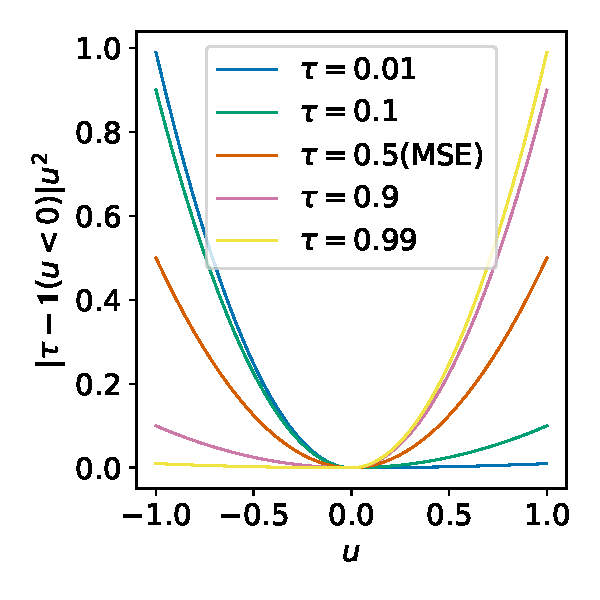
\includegraphics[width=\textwidth]{images/expectile_loss.pdf}
\end{subfigure}
\begin{subfigure}[t]{0.32\textwidth}
    \centering
    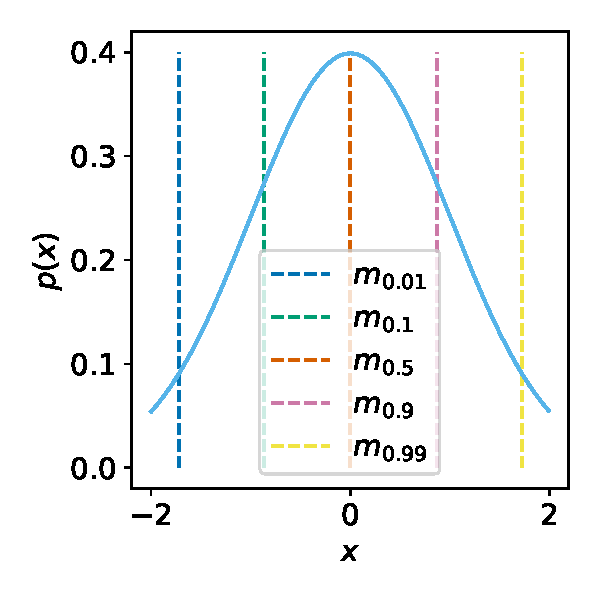
\includegraphics[width=\textwidth]{images/expectile_normal.pdf}
\end{subfigure}
\begin{subfigure}[t]{0.32\textwidth}
    \centering
    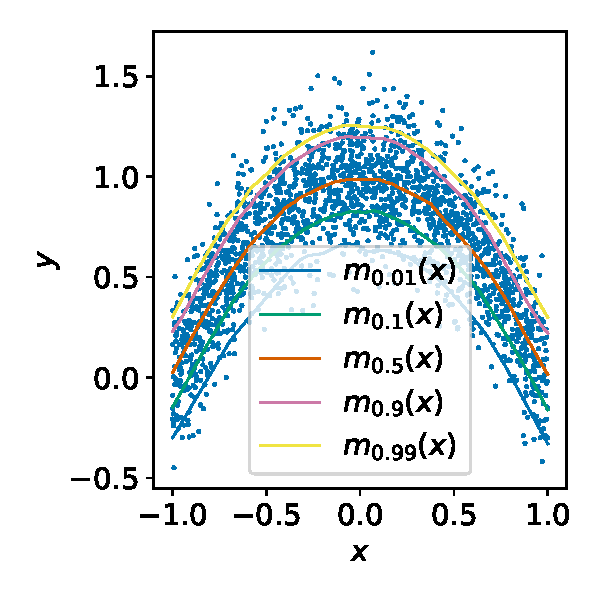
\includegraphics[width=\textwidth]{images/expectile_regression.pdf}
\end{subfigure}
\caption{\textbf{Left:} The asymmetric squared loss used for expectile regression. $\tau=0.5$ corresponds to the standard mean squared error loss, while $\tau=0.9$ gives more weight to positives differences.
\textbf{Center:} Expectiles of a normal distribution.
    \textbf{Right:} an example of estimating state conditional expectiles of a two-dimensional random variable. Each $x$ corresponds to a distribution over $y$. We can approximate a maximum of this random variable with expectile regression: $\tau=0.5$ correspond to the conditional mean statistics of the distribution, while $\tau \approx 1$ approximates the maximum operator over in-support values of $y$.\label{fig:expectiles}}
\end{figure}

% Note that the only difference between expectile and quantile regression is that we use asymmetric L2 loss instead of asymmetric L1 loss. In early experiments, we used L1 loss; however, we found expectile regression to perform better.


We can also use this formulation to predict expectiles of a conditional distribution:
$$\argmin_{m_\tau(x)} \E_{(x,y)\sim \D}[L_2^\tau(y-m_\tau(x))].$$
\Cref{fig:expectiles} (right) illustrates conditional expectile regression on a simple two-dimensional distribution. Note that we can optimize this objective with stochastic gradient descent. It provides unbiased gradients and is easy to implement with standard machine learning libraries. 


\subsection{Learning the Value Function with Expectile Regression}

Expectile regression provides us with a powerful framework to estimate statistics of a random variable beyond mean regression. We can use expectile regression to modify the policy evaluation objective in \Cref{eqn:td_sarsa} to predict an upper expectile of the TD targets that approximates the maximum of $r(s,a) + \gamma Q_{\hat{\theta}}(s',a')$ over actions $a'$ constrained to the dataset actions, as in \Cref{eqn:bq_learning}.
This leads to the following expectile regression objective:
\begin{align*}
&L(\theta)=\E_{(s,a,s',a')\sim\D}[L_2^\tau(r(s,a) + \gamma Q_{\hat{\theta}}(s', a')- Q_\theta(s,a))].
\end{align*}
%%SL.9.28: It might not actually be completely obvious to readers what this is doing -- can you more explicitly explain which max this is estimating. 
However, this formulation has a significant drawback. Instead of estimating expectiles just with respect to the actions in the support of the data, it also incorporates stochasticity that comes from the environment dynamics $s'\sim p(\cdot|s,a)$. Therefore, a large target value might not necessarily reflect the existence of a single action that achieves that value, but rather a ``lucky'' sample that happened to have transitioned into a good state.
We resolve this by introducing a separate value function that approximates an expectile only with respect to the action distribution, leading to the following loss:
\begin{equation}
    \label{eqn:fit_v}
    L_V(\psi) = \E_{(s,a)~\sim \D}[L_2^\tau(Q_{\hat{\theta}}(s,a) - V_\psi(s))].
\end{equation}
We can then use this estimate to update the $Q$-functions with the MSE loss, which averages over the stochasticity from the transitions and avoids the ``lucky'' sample issue mentioned above:
\begin{equation}
    \label{eqn:fit_q}
    L_Q(\theta) = \E_{(s,a,s')~\sim \D}[(r(s,a) + \gamma V_\psi(s') - Q_{\theta}(s,a))^2].
\end{equation}
Note that these losses do not use any explicit policy, and only utilize actions from the dataset for both objectives, similarly to SARSA-style policy evaluation.
%%SL.10.3: Maybe forward reference the theory and say:
In \Cref{sec:analysis}, we will show that this procedure recovers the optimal Q-function under some assumptions. Also, even though only one action is available for every state in the dataset for continuous action spaces, due to neural network generalization, the expectile regression does not result in SARSA-style policy evaluation as shown in \Cref{sec:exp_comparisons}.

\subsection{Policy Extraction and Algorithm Summary}

\begin{wrapfigure}{R}{0.35\textwidth}
    \begin{minipage}{0.35\textwidth}
        \begin{algorithm}[H]
            \caption{\Ournamepref Q-learning}
            %%SL.9.28: Rules about capitalization: if using title case, then capitalize all words (including the word after "-" -- i.e., In-Sample Q-Learning); if using sentence case, then capitalize only the first word, i.e., In-sample Q-learning.
            \begin{algorithmic}
            \label{alg:iql}
                \State Initialize parameters $\psi$, $\theta$, $\hat{\theta}$, $\phi$.
                \State TD learning (IQL):
                \For{each gradient step}
                \State $\psi \leftarrow \psi - \lambda_V \nabla_\psi L_V(\psi)$ 
                \State $\theta \leftarrow \theta - \lambda_Q \nabla_{\theta} L_Q(\theta)$
                \State $\hat{\theta} \leftarrow (1-\alpha)\hat{\theta} + \alpha\theta$
                \EndFor
                \State Policy extraction (AWR):
                \For{each gradient step}
                \State $\phi \leftarrow \phi - \lambda_\pi \nabla_\phi L_\pi(\phi)$
                \EndFor
            \end{algorithmic}
        \end{algorithm}
    \end{minipage}
\end{wrapfigure}
%%SL.9.28: Try to tweak the spacing a bit so that the whitespace around this pseudocode is not so gigantic.

While our modified TD learning procedure learns an approximation to the optimal Q-function, it does not explicitly represent the corresponding policy, and therefore requires a separate policy extraction step. While one can consider any technique for policy extraction that constrains the learned policy to stay close to the dataset actions,
% in the spirit of preserving simplicity and efficiency,
we aim for a simple method for policy extraction. As before, we aim to avoid using out-of-samples actions. Therefore, we extract the policy with advantage-weighted regression~\citep{peters2007reinforcement, peng2019advantage} previously successfully used for policy extraction in Offline RL~\citep{wang2018exponentially,nair2020awac, brandfonbrener2021offline}:
\begin{equation}
    L_\pi(\phi) = \E_{(s,a)~\sim \D}[\exp(\beta(Q_{\hat{\theta}}(s,a) - V_\psi(s)))\log \pi_\phi(a|s)],
    \label{eqn:awr}
\end{equation}
where $\beta \in [0, \infty)$  is an inverse temperature. % For smaller hyperparameter values, the objective behaves similarly to behavioral cloning, while for larger values, it attempts to recover the maximum of the $Q$-function.
Note that this objective does not clone all actions from the dataset but, as shown in prior work, this objective learns a policy that maximizes the $Q$-values subject to a distribution constraint~\citep{peters2007reinforcement,peng2019advantage,nair2020awac}. This step can be seen as selecting and cloning the most optimal actions in the dataset.
%%SL.9.28: Perhaps add a short sentence or two explaining what this does, with a reference to prior work? Otherwise readers might be confused and think that this is basically a heuristic that doesn't mean anything, if they are not familiar with the prior work

Our final algorithm consists of two stages. First, we fit the value function and $Q$, performing a number of gradient updates alternating between Eqn.~(\ref{eqn:fit_v}) and (\ref{eqn:fit_q}). Second, we perform stochastic gradient descent on \Cref{eqn:awr}.
For both steps, we use a version of clipped double Q-learning~\citep{fujimoto2018addressing}, taking a minimum of two $Q$-functions for $V$-function and policy updates.
We summarize our final method in \Cref{alg:iql}. Note that the policy does not influence the value function in any way, and therefore extraction could be performed either concurrently or after TD learning. Concurrent learning provides a way to use \ourname with online finetuning, as we discuss in \Cref{sec:finetune}.

\subsection{Analysis}

\label{sec:analysis}

%%SL.10.3: My suggestion would be to shorten this to make space for more experiment details. Consider stating the main theorem result, and providing a proof sketch that conveys some intuition, with most of the proof in an appendix

In this section, we will show that \ourname can recover the optimal value function under the dataset support constraints.
First, we prove a simple lemma that we will then use to show how our approach can enable learning the optimal value function.
\begin{lemma}
\label{lem:1}
Let $X$ be a real-valued random variable with a bounded support
%%SL.9.28: There is a terminology confusion here. "Range" could literally mean the range of the value (e.g., the range of Q(s,a) is [0, Rmax/(1-gamma)]). But you do not want the max of the range, you want the maximum value with non-zero probability! That is much more subtle, but this distinction is very important for showing the correctness of your method later.
%%Ilya.9.29: Changed to support.
and supremum of the support is $x^*$. Then,
\vspace{-0.2cm}
$$
\lim_{\tau\rightarrow1} m_\tau = x^*
$$
\end{lemma}
\begin{sproof}
\vspace{-0.2cm}
One can show that expectiles of a random variable have the same supremum $x^*$. Moreover, for all $\tau_1$ and $\tau_2$ such that $\tau_1 < \tau_2$, we get $m_{\tau_1} \le m_{\tau_2}$. Therefore, the limit follows from the properties of bounded monotonically non-decreasing functions.
\end{sproof}

In the following theorems, we show that under certain assumptions, our method indeed approximates the optimal state-action value $Q^*$ and performs multi-step dynamical programming.
% For the same of simplicity we consider tabular MDPs.
%%SL.9.28: Add a few sentences to ease the reader into this, e.g.:
We first prove a technical lemma relating different expectiles of the Q-function, and then derive our main result regarding the optimality of our method.
% Also, did you already introduce this V_\tau style notation?

For the sake of simplicity, we introduce the following notation for our analysis. Let $\E^\tau_{x\sim X}[x]$ be a $\tau^\text{th}$ expectile of $X$ (e.g., $\E^{0.5}$ corresponds to the standard expectation). Then, we define $V_{\tau}(s)$ and $Q_\tau(s, a)$, which correspond to optimal solutions of Eqn. \ref{eqn:fit_v} and \ref{eqn:fit_q} correspondingly, recursively as:
\begin{align*}
    V_\tau(s) &= \E^\tau_{a\sim \pi_\beta(\cdot|s)} [Q_\tau(s, a)], \\
    Q_\tau(s,a)&=r(s,a)+\gamma\E_{s'\sim p(\cdot|s,a)}[V_\tau(s')].
\end{align*}


\begin{lemma}
\label{lem:2}
For all $s$, $\tau_1$ and $\tau_2$ such that $\tau_1 < \tau_2$ we get
$V_{\tau_1}(s) \le V_{\tau_2} (s)$.
\end{lemma}
%%SL.9.28: I think these "wall of algebra" proofs can be deferred to an appendix to make the paper more readable
\begin{proof}
The proof follows the policy improvement proof~\citep{sutton2018reinforcement}. See \Cref{app:proofs}.
\end{proof}

\label{sec:iql}
\begin{corollary}
For any $\tau$ and $s$ we have
$
V_\tau(s)\le\max_{\substack{a\in \A \\\text{s.t. }\pi_\beta(a|s) > 0}}Q^*(s,a)
$
where $V_\tau(s)$ is defined as above and $Q^*(s,a)$ is an optimal state-action value function constrained to the dataset and defined as
\vspace{-0.4cm}
$$
Q^*(s, a) = r(s,a) + \gamma \E_{s'\sim p(\cdot|s,a)}\left[\max_{\substack{a'\in \A \\\text{s.t. }\pi_\beta(a'|s') > 0}}Q^*(s',a')\right].
$$
\vspace{-0.5cm}
\label{theorem:cor}
\end{corollary}
\vspace{-0.2cm}
\begin{proof}
The proof follows from the observation that convex combination is smaller than maximum.
\end{proof}
\begin{theorem}
\label{theorem:iql}
$$
\lim_{\tau \rightarrow 1} V_\tau(s) = \max_{\substack{a\in \A \\\text{s.t. }\pi_\beta(a|s) > 0}}Q^*(s,a).
$$
\vspace{-0.5cm}
\end{theorem}
\begin{proof}
Follows from combining Lemma \ref{lem:1} and  \Cref{theorem:cor}.
\end{proof}
Therefore, for a larger value of $\tau < 1$, we get a better approximation of the maximum. On the other hand, it also becomes a more challenging optimization problem. Thus, we treat $\tau$ as a hyperparameter.
Due to the property discussed in \Cref{theorem:iql} we dub our method implicit Q-learning (\ourname). We also emphasize that our value learning method defines the entire spectrum of methods between SARSA ($\tau=0.5$) and Q-Learning ($\tau \rightarrow 1$). Note that in contrast to other multi-step methods, IQL absorbs the policy improvement step into value learning. Therefore, fitting Q-function corresponds to the policy evaluation step, while fitting the value function with IQL corresponds to \textit{implicit} policy improvement.

%%SL.9.28: As per our discussion before, would it be possible to add a more complete theorem that quantifies the error we get from using tau < 1? In general, I think this section would be more compelling if we have a bit more discussion of the takeaways and more convincingly articulate that this algorithm will converge to the optimal policy. It would also help if we are more explicit about what the constraint on the max really means, and state it formally (e.g., is it a support constraint? what is the set of a precisely? and why is that true?)

\section{Experimental Evaluation}

\vspace{-0.4cm}

%We evaluate the performance of our method on a variety of offline RL tasks, ranging from didactic examples on gridworlds to high-dimensional benchmarks. We aim to evaluate how our method compares to prior work, and whether our approach can perform multi-step dynamic programming and estimate a near-optimal value function using only the actions in the dataset. We first evaluate our algorithm on a simple maze environment to illustrate the difference between our approach one-step policy improvement~\citep{brandfonbrener2021offline}.
%Then, we evaluate our approach against prior state-of-the-art methods on D4RL~\citep{fu2020d4rl}, a standard benchmark for offline reinforcement learning.
%%SL.9.20: I might recommend trying to explicitly state your research questions and hypotheses at the top of the experiments to make it clear to the reader what to expect. That might be especially effective in your case to put the didactic illustrative example into the context of your broader research questions and claims.
%%SL.10.3: Here is a way we could make this paragraph more interesting (I'm putting it here in a comment, and you can decide whether this phrasing makes sense or not):
Our experiments aim to evaluate our method comparatively, in contrast to prior offline RL methods, and in particular to understand how our approach compares both to single-step methods and multi-step dynamic programming approaches. We will first demonstrate the benefits of multi-step dynamic programming methods, such as ours, in contrast to single-step methods, showing that on some problems this difference can be extremely large. We will then compare \ourname with state-of-the-art single-step and multi-step algorithms on the D4RL~\citep{fu2020d4rl} benchmark tasks, studying the degree to which we can learn effective policies using only the actions in the dataset. We examine domains that contain near-optimal trajectories, where single-step methods perform well, as well as domains with no optimal trajectories at all, which require multi-step dynamic programming. Finally, we will study how \ourname compares to prior methods when finetuning with online RL starting from an offline RL initialization.

\vspace{-0.2cm}
\subsection{The Difference Between One-Step Policy Improvement and \ourname}
\label{sec:example}
\vspace{-0.2cm}


We first use a simple maze environment to illustrate the importance of multi-step dynamic programming for offline RL.
%%SL.9.28: not 100% obvious what this has to do with our method
% difference between Onestep Policy Improvement~\citep{brandfonbrener2021offline, wang2018exponentially}
%%SL.9.20: I'm not sure "SARSA" is an accurate characterization of this method. SARSA is really a policy evaluation procedure, whereas what you are describing is a bit different. I might recommend proposing a name for such methods earlier in the paper and just using that name (maybe single-step methods or something?). Also, I would recommend to cite *all* the methods that do that together, rather than just one.
% and \ourname on a fixed dataset.
%%SL.9.20: [METHODNAME]. 
The maze has a u-shape, a single start state, and a single goal state (see \Cref{fig:umaze}).
The agent receives a reward of 10 for entering the goal state and zero reward for all other transitions. With a probability of $0.25$, the agent transitions to a random state, and otherwise to the commanded state.
The dataset consists of 1 optimal trajectory and 99 trajectories with uniform random actions.
%%SL.9.20: Some of the above design decisions for this task come off as a bit arbitrary. It would likely be clearer to the reader what is going on if the beginning of this paragraph more clearly lays out the motivation from which these design decisions stem. Also, remember that you don't have to exhaustively present every detail, you could just as well defer some of the details to an appendix and just cover enough details so that readers understand what you're doing and appreciate the end result.
Due to a short horizon of the problem, we use $\gamma=0.9$.


\begin{figure}
\begin{subfigure}{0.233\textwidth}
    \centering
    
\includegraphics[width=0.8\textwidth]{images/maze/umaze.png}
    \caption{toy maze MDP \label{fig:umaze}}
\end{subfigure}%
\hspace{0.01mm}
\begin{subfigure}{0.235\textwidth}
    \centering
    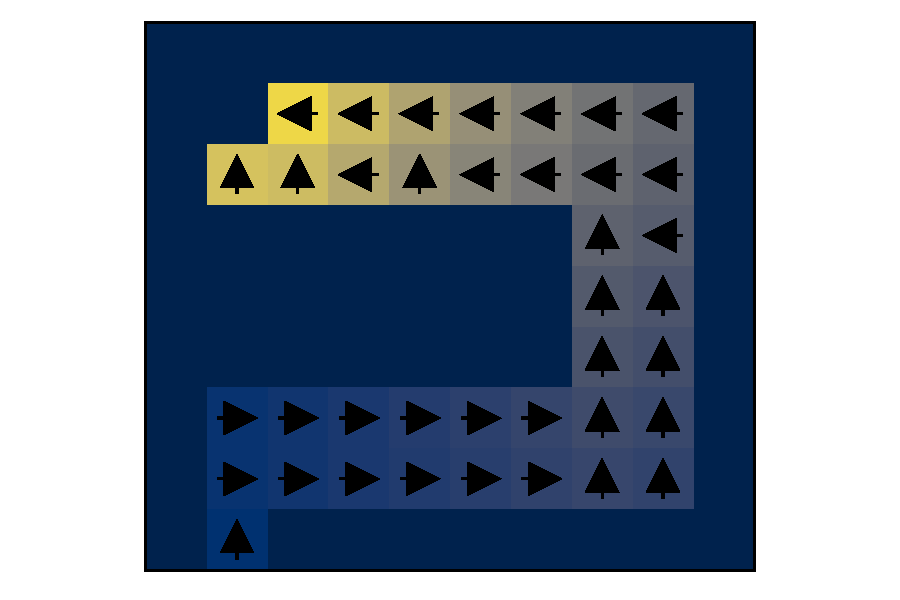
\includegraphics[width=0.8\textwidth]{images/maze/umaze_ql.pdf}
    \caption{true optimal $V^\star$}
\end{subfigure}%
\hspace{0.01mm}
\begin{subfigure}{0.235\textwidth}
    \centering
    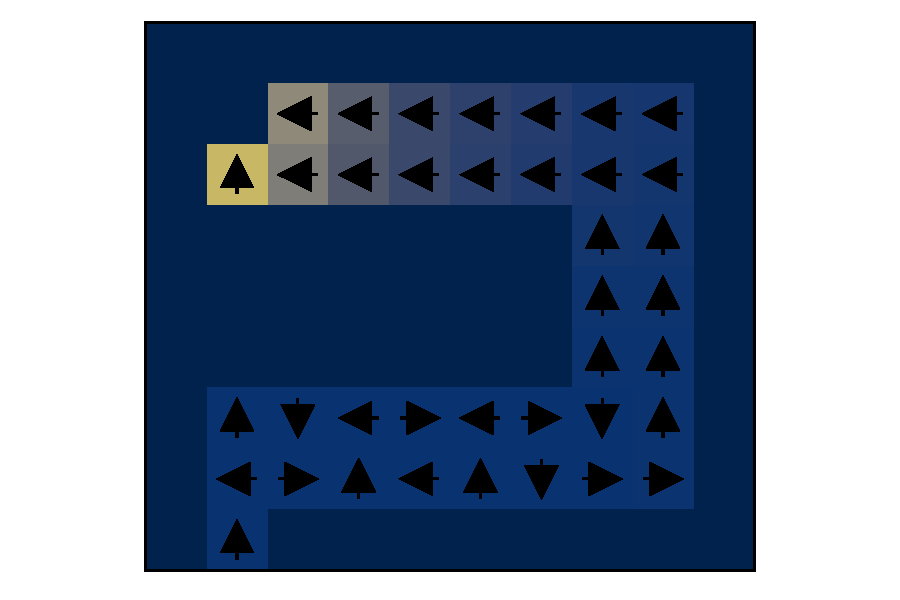
\includegraphics[width=0.8\textwidth]{images/maze/maze_2.pdf}
    \caption{One-step Policy Eval.}
    %%SL.10.3: should this rather be called "one-step policy evaluation" or "single-step method" or something? (whichever terminology you decide to use, but let's just be consistent about it)
\end{subfigure}%
\begin{subfigure}{0.28\textwidth}
    \centering
    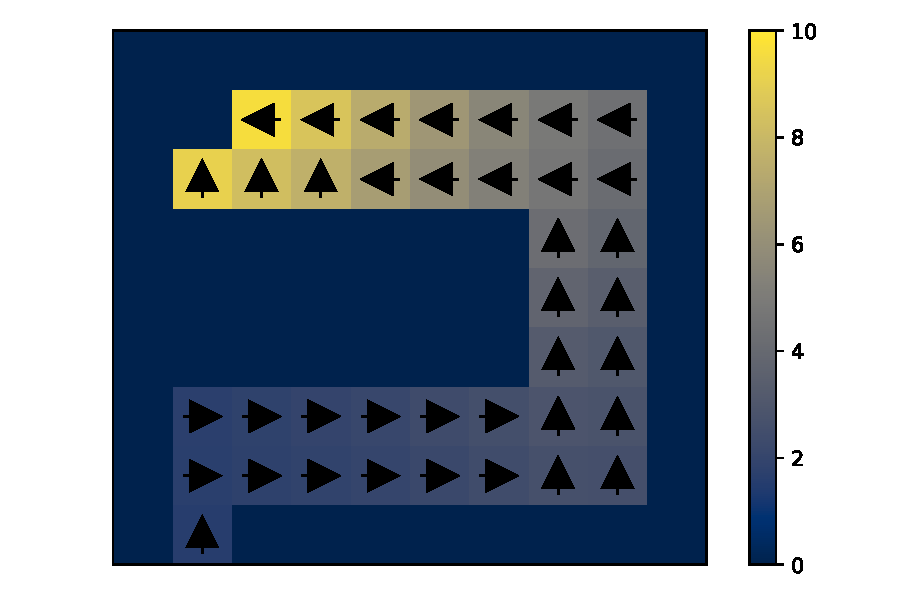
\includegraphics[width=0.8\textwidth]{images/maze/maze_1.pdf}
    \caption{\ourname}
\end{subfigure}
\caption{Evaluation of our algorithm on a toy umaze environment (a).
%%SL.9.28: make it clear what is being visualized (the value function)
When the static dataset is heavily corrupted by suboptimal actions, one-step policy evaluation
%%SL.10.3: we should pick a term for this and use it throughout (whether it's one-step policy evaluation, single-step, whatever -- any term is fine, and I actually think one-step policy evaluation (OSPE?) is a good choice, we should just be very consistent about it and clearly define it at the beginning)
results in a value function that degrades to zero far from the rewarding states too quickly (c). Our algorithm aims to learn a near-optimal value function, combining the best properties of SARSA-style evaluation with the ability to perform multi-step dynamic programming, leading to value functions that are much closer to optimality (shown in (b)) and producing a much better policy (d).\label{fig:illustratiev}}
%%SL.9.20: See my earlier point about abuse of the term "SARSA". I also wouldn't call it an "evaluation", as it's really more of an illustration.
%%SL.9.28: could we also add the ground truth value function as (d), and then show that our method learns a value function that matches the true one? this would also make the figure smaller since adding a 4th plot on the right would shrink it vertically
\end{figure}


\Cref{fig:illustratiev} (c, d) % illustrates the difference between
%%SL.10.3: 
illustrates the difference between single-step methods which fit $Q^\pi(s,a)$ via SARSA-style objective, in this case represented by 
Onepstep RL~\citep{brandfonbrener2021offline, wang2018exponentially, gulcehre2021regularized} and \ourname with $\tau=0.95$. Note that these methods represent a special case of our method with $\tau=0.5$.
% These one-step methods estimate the $Q$-values according to the behavior policy, and since the behavior policy takes many suboptimal random actions, the resulting value will significantly underestimate the true value function. In this case, it leads to the signal vanishing over time;
%%SL.9.28: need to fix the above, maybe rephrase like this:
Although states closer to the high reward state will still have higher values, these values decay much faster as we move further away than they would for the optimal value function, and the resulting policy is highly suboptimal.
% After several steps, the value is dominated by noise instead of long-term optimality. As a result, the $Q$-function can no longer produce optimal actions anymore.
Since \ourname (d) performs iterative dynamic programming, it correctly propagates the signal, and the values are no longer dominated by noise. The resulting value function closely matches the true optimal value function (b).
%%SL.9.20: Generally, I think a didactic example like this is great to have, but I think the current example will come across as rather confusing to some readers. There are multiple distinct things going on here, such as the noisy rewards, the horizon, the nature of the data distribution, etc., and some readers might understandably wonder which of these matter more or less. But that's all a distraction: the point is to illustrate that single-step methods *in principle* can do very poorly, and therefore should not be relied upon. At the same time, our method can in fact perform full dynamic programming, despite having the "structure" of a single-step method. We should lay out the goals of this didactic example clearly at the beginning of the paragraph, and try to minimize "distracting" details that are not strictly necessary to understand the main outcome.
%%SL.9.20: Additionally, I think it would be *really* nice if this experiment also confirms that numerically the values learned by our method actually match the real values (if indeed they do), which would serve to empirically back up our (soon to be added?) theoretical claim that the method converges to the optimal value function in the absence of approximation errors


% \subsection{Implementation details}

\vspace{-0.2cm}
\subsection{Comparisons on Offline RL Benchmarks}
\vspace{-0.2cm}
\label{sec:exp_comparisons}

\begin{table}[t]\centering
%%SL.9.20: it would be nice to add some other methods, otherwise it will seem arbitrary that we picked only these particular methods to compare.
\begin{threeparttable}
\caption{Averaged normalized scores on MuJoCo locomotion and Ant Maze tasks. Our method outperforms prior methods on the challenging Ant Maze tasks, which require dynamic programming, and is competitive with the best prior methods on the locomotion tasks.  %We measure runtime for our reimplementations in JAX, which are faster than the original implementations, for all methods except Decision Transformers (DT). For DT, we take numbers reported by \cite{fujimoto2021minimalist}.
}\label{tab:d4rl}
%Please add the following packages if necessary:
%\usepackage{booktabs, multirow} % for borders and merged ranges
%\usepackage{soul}% for underlines
%\usepackage[table]{xcolor} % for cell colors
%\usepackage{changepage,threeparttable} % for wide tables
%If the table is too wide, replace \begin{table}[!htp]...\end{table} with
%\begin{adjustwidth}{-2.5 cm}{-2.5 cm}\centering\begin{threeparttable}[!htb]...\end{threeparttable}\end{adjustwidth
%Please add the following packages if necessary:
%\usepackage{booktabs, multirow} % for borders and merged ranges
%\usepackage{soul}% for underlines
%\usepackage[table]{xcolor} % for cell colors
%\usepackage{changepage,threeparttable} % for wide tables
%If the table is too wide, replace \begin{table}[!htp]...\end{table} with
%\begin{adjustwidth}{-2.5 cm}{-2.5 cm}\centering\begin{threeparttable}[!htb]...\end{threeparttable}\end{adjustwidth}
\tiny
\begin{tabular}{l||rrrrrrrrr|r}
Dataset &BC &10\%BC & BCQ &DT & ABM &AWAC &Onestep RL &TD3+BC &CQL & \ourname (Ours) \\\hline
halfcheetah-m-v2 &42.6 &42.5 & \textbf{47.0} & 42.6$\pm$0.1 & 53.6 & 43.5 &\textbf{48.4$\pm$0.1} &\textbf{48.3$\pm$0.3} &44.0$\pm$5.4 &\textbf{47.4$\pm$0.2} \\
hopper-m-v2 &52.9 &56.9 & 56.7 &\textbf{67.6$\pm$1.0} & 0.7 &57.0 &$59.6\pm$2.5 &59.3$\pm$4.2 &58.5$\pm$2.1 &\textbf{66.2$\pm$5.7} \\
walker2d-m-v2 &75.3 &75.0 & 72.6 &74.0$\pm$1.4 & 0.5 & 72.4 &\textbf{81.8$\pm$2.2} &83.7$\pm$2.1 &72.5$\pm$0.8 &78.3$\pm$ 8.7\\
halfcheetah-m-r-v2 &36.6 &40.6 & 40.4 &36.6$\pm$0.8 & \textbf{50.5} & 40.5 &38.1$\pm$1.3 &\textbf{44.6$\pm$0.5} &\textbf{45.5$\pm$0.5} &\textbf{44.2$\pm$1.2} \\
hopper-m-r-v2 &18.1 &75.9 &53.3 &82.7$\pm$7.0 & 49.6 &37.2 &\textbf{97.5$\pm$0.7} &60.9$\pm$18.8 &\textbf{95.0$\pm$6.4} &\textbf{94.7$\pm$8.6} \\
walker2d-m-r-v2 &26.0 &62.5 & 52.1 &66.6$\pm$3.0 & 53.8 & 27.0 &49.5$\pm$12.0 &\textbf{81.8$\pm$5.5} &77.2$\pm$5.5 &73.8$\pm$7.1 \\
halfcheetah-m-e-v2 &55.2 &\textbf{92.9} &\textbf{89.1} &86.8$\pm$1.3 & 18.5 & 42.8 &
\textbf{93.4$\pm$1.6} &\textbf{90.7$\pm$4.3} &\textbf{91.6$\pm$2.8} &86.7$\pm$5.3 \\
hopper-m-e-v2 &52.5 &\textbf{110.9} & 81.8 &\textbf{107.6$\pm$1.8} & 0.7 & 55.8 &103.3$\pm$1.9 &98.0$\pm$9.4 &\textbf{105.4$\pm$6.8} &91.5$\pm$14.3 \\
walker2d-m-e-v2 &\textbf{107.5} &\textbf{109.0} & \textbf{109.5}&\textbf{108.1$\pm$0.2} & 3.5 & 74.5 &\textbf{113.0$\pm$0.4} &\textbf{110.1$\pm$0.5} &\textbf{108.8$\pm$0.7} &\textbf{109.6$\pm$1.0} \\ \hline
locomotion-v2 total &466.7 &\textbf{666.2} & 602.5 &\textbf{672.6$\pm$16.6} & 231.4 & 450.7 &\textbf{684.6$\pm$22.7} &\textbf{677.4$\pm$44.5} &\textbf{698.5$\pm$31.0} &\textbf{692.4$\pm$52.1} \\ \hline
antmaze-u-v0 &54.6 &62.8 &\textbf{89.8} &59.2 & 59.9 &56.7 &64.3 &78.6 &74.0 &\textbf{87.5 $\pm$ 2.6} \\
antmaze-u-d-v0 &45.6 &50.2 & \textbf{83.0} &53.0 & 48.7 & 49.3 &60.7 &71.4 &\textbf{84.0} &62.2 $\pm$ 13.8 \\
antmaze-m-p-v0 &0.0 &5.4 & 15.0 &0.0 & 0.0 &0.0 &0.3 &10.6 &61.2 &\textbf{71.2 $\pm$ 7.3} \\
antmaze-m-d-v0 &0.0 &9.8 & 0.0 &0.0 & 0.5 &0.7 &0.0 &3.0 &53.7 &\textbf{70.0 $\pm$ 10.9} \\
antmaze-l-p-v0 &0.0 &0.0 & 0.0 &0.0 & 0. & 0.0 &0.0 &0.2 &15.8 &\textbf{39.6$\pm$5.8} \\
antmaze-l-d-v0 &0.0 &6.0 & 0.0 &0.0 & 0.0 & 1.0 &0.0 &0.0 &14.9 &\textbf{47.5$\pm$9.5} \\ \hline
antmaze-v0 total &100.2 &134.2 &187.8 &112.2 & 109.1 & 107.7 &125.3 &163.8 &303.6 &\textbf{378.0$\pm$49.9} \\ 
\hline \hline
total &566.9 &800.4& 790.3 &784.8 & 340.5 & 558.4 &809.9 &841.2 &1002.1 &\textbf{1070.4$\pm$102.0} \\
\hline \hline
kitchen-v0 total & \textbf{154.5} & - & - & - & - & - & - & - & 144.6 & \textbf{159.8$\pm$22.6} \\
adroit-v0 total & 104.5 & - & - & - & - & - & - & - & 93.6 & \textbf{118.1$\pm$30.7} \\
\hline \hline
total+kitchen+adroit &825.9 & - & - & - & - & - & - & - & 1240.3 &\textbf{1348.3$\pm$155.3} \\
\hline
runtime & 10m & 10m &  & 960m & & 20m & 20m$^*$ & 20m & 80m & 20m
\end{tabular}
\begin{tablenotes}
\item $^*$: Note that it is challenging to compare one-step and multi-step methods directly. Also, \cite{brandfonbrener2021offline} reports results for a set of hyperparameters, such as batch and network size, that is significantly different from other methods. We report results for the original hyperparameters and runtime for a comparable set of hyperparameters.
% Note that it corresponds to marginally worse performance.
%%SL.9.28: Try to find some other place to stick this footnote. It's rather delicate too -- I think it's easy for readers to misunderstand what this footnote means. Perhaps make it a proper footnote (rather than a huge block of text in the caption), and reference an appendix where you can explain this distinction in detail so that there is a full explanation for any curious reader. Also, what do you mean by hyperparameters? Do they use hyperparameters that are per-task or something? The way this is written right now, it makes it sound like the comparison is unfair to this prior method.
%%SL.10.3: OK, this discussion is a bit better, but it still sounds a little unfair, like we intentionally used worse hyperparameters -- can we also present the hyperparameters that they use?
%%Ilya: We used good hyper params for the results and bad for runtime. I will remove the bit about performance. I think it will be less confusing about it.
\end{tablenotes}
\end{threeparttable}
% \vspace{-0.5cm}
\end{table}

\begin{wrapfigure}{R}{0.5\textwidth}
    % \vspace{-0.6cm}
    \centering
    %%SL.10.3: This figure is analyzed later than Table 1, can we mess with latex figure placement and somehow get this to appear at the bottom and the table at the top?
    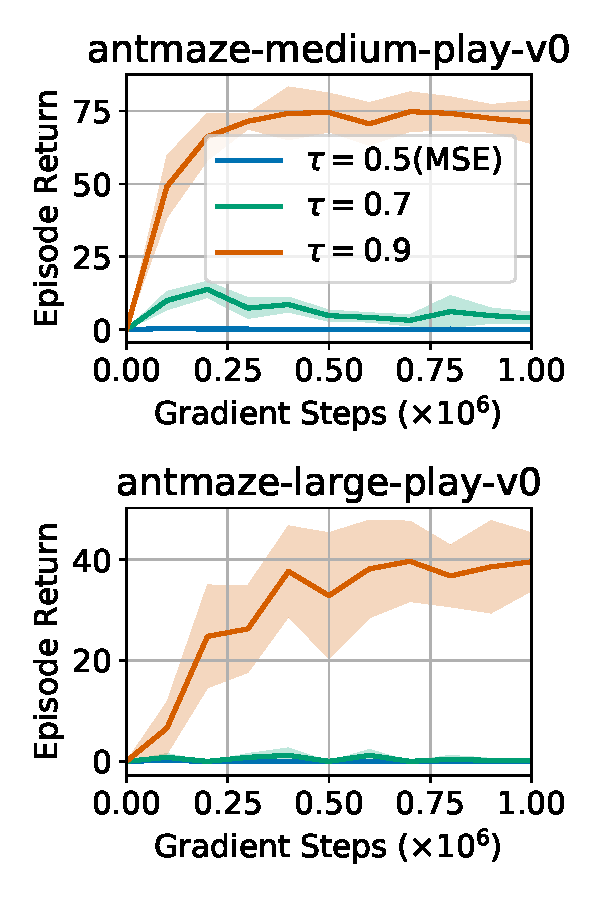
\includegraphics[width=0.24\textwidth]{images/antmaze_rebuttal.pdf}
    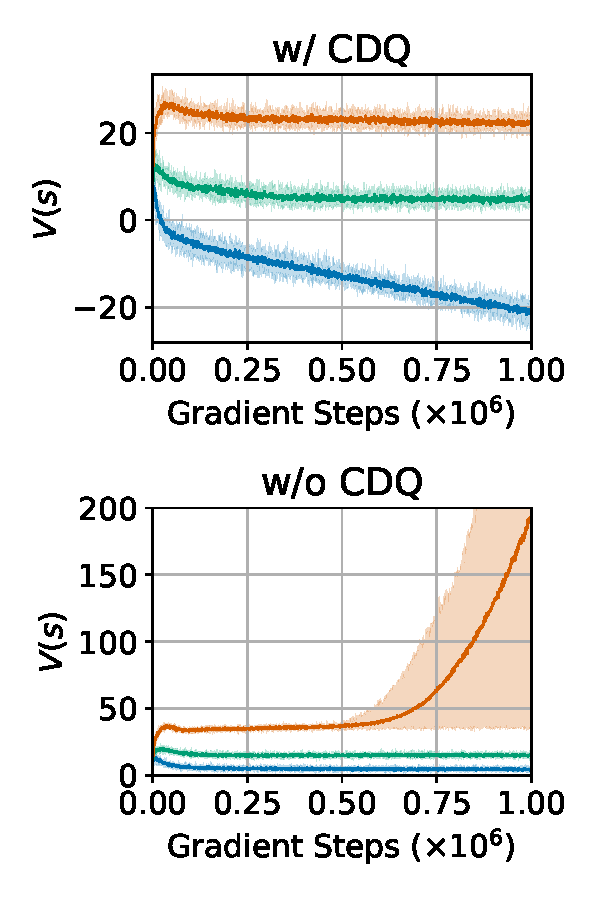
\includegraphics[width=0.24\textwidth]{images/antmaze_values_cdq.pdf}
    \caption{\textbf{Left}: Estimating a larger expectile $\tau$ is crucial for antmaze tasks that require dynamical programming ('stitching'). 
 \textbf{Right:} Clipped double Q-Learning (CDQ) is crucial for learning values for $\tau=0.9$.
    %IQL with $\tau=0.5$
    % which corresponds to Onestep RL \citep{brandfonbrener2021offline}
    %is not able to propagate the signal A larger expectile $\tau=0.9$ reaches the state-of-the-art performance on the tasks.
    }
    % \vspace{-0.6cm}
    %%SL.9.20: I think having a more thorough examination of ant maze in particular like this makes sense, but I think readers will want to then see more methods in the graphs. Basically, right now this looks like an ablation, but it's actually a comparative result in disguise (as evidenced by the caption). I think you should pick one or the other, rather than leaning so heavily on the Onestep RL <=> tau=0.5 equivalence (which strikes me as a bit confusing anyway).
    %%SL.10.3: If we end up being short on space, I think it would also be fine to make this a table. It's size is a bit out of proportion with its importance right now.
    \label{fig:antmaze}
\end{wrapfigure}

Next, we evaluate our approach on the D4RL benchmark in comparison to prior methods (see \Cref{tab:d4rl}).
The MuJoCo tasks in D4RL consist of the Gym locomotion tasks, the Ant Maze tasks, and the Adroit and Kitchen robotic manipulation environments. Some prior works, particularly those proposing one-step methods, focus entirely on the Gym locomotion tasks. However, these tasks include a significant fraction of near-optimal trajectories in the dataset. In contrast, the Ant Maze tasks, especially the medium and large ones, contain very few or no near-optimal trajectories, making them very challenging for one-step methods. These domains require ``stitching'' parts of suboptimal trajectories that travel between different states to find a path from the start to the goal of the maze~\citep{fu2020d4rl}. As we will show, multi-step dynamic programming is essential in these domains. The Adroit and Kitchen tasks are comparatively less discriminating, and we found that most RL methods perform similarly to imitation learning in these domains~\citep{florence2021implicit}. We therefore focus our analysis on the Gym locomotion and Ant Maze domains, but include full Adroit and Kitchen results in \Cref{app:experiments} for completeness.

\vspace{-0.15in}
\paragraph{Comparisons and baselines.} We compare to methods that are representative of both multi-step dynamic programming and one-step approaches. In the former category, we compare to CQL~\citep{kumar2020conservative}, TD3+BC~\citep{fujimoto2021minimalist}, and AWAC~\citep{nair2020awac}. In the latter category, we compare to Onestep RL~\citep{brandfonbrener2021offline} and Decision Transformers~\citep{chen2021decision}. We obtained the Decision Transformers results on Ant Maze subsets of D4RL tasks using the author-provided implementation\footnote{https://github.com/kzl/decision-transformer} and following authors instructions communicated over email. We obtained results for TD3+BC and Onestep RL (Exp. Weight) directly from the authors. Note that \citet{chen2021decision} and \citet{brandfonbrener2021offline}
%%SL.9.28: should this also include TD3+BC?
%%Ilya: TD3+BC has correct comparisons. They just omit comparisons on -v2
incorrectly report results for some prior methods, such as CQL, using the ``-v0'' environments. These generally produce lower scores than the ``-v2'' environments that these papers use for their own methods. We use the ``-v2'' environments for all methods to ensure a fair comparison, resulting in higher values for CQL. Because of this fix, our reported CQL scores are higher than all other prior methods. We obtained results for ``-v2'' datasets using an author-suggested implementation.\footnote{https://github.com/young-geng/CQL}
% In particular, we focus on two sets of tasks from the benchmark: the widely used MuJoCo locomotion tasks, and the Ant Maze tasks.
%%SL.10.3: It still comes across as a little arbitrary (see my comment on Slack, which I'll send shortly)
% The latter are particularly challenging for offline RL algorithms that do not perform multi-step dynamic programming, because on the harder mazes, the dataset has few or no trajectories that traverse a full path from the start to the goal. Instead, offline RL methods must stitch together different parts of suboptimal trajectories between different start-goal pairs in order to recover near-optimal behavior~\citep{fu2020d4rl}.
% \ourname performs better or similarly to prior methods on MuJoCo locomotion task.
% However, \ourname significantly outperforms the prior work on Ant Maze tasks that cannot be solved by imitation learning that further demonstrates the effectiveness of our approach for Offline RL. We provide further details, including additional results and hyperparameters, in \Cref{app:experiments}.
%%SL.10.3: Given that this is our main result, I feel like we need to expand on the discussion here a lot more. Definitely it would be good to move "Comparisons and baselines" discussion from Appendix B back in here. Perhaps we can add some discussion along these lines:
%
On the Gym locomotion tasks (halfcheetah, hopper, walker2d), we find that \ourname performs comparably to the best performing prior method, CQL. On the more challenging Ant Maze task, \ourname outperforms CQL, and outperforms the one-step methods by a very large margin.
%Note also that the total runtime of \ourname is about 4x lower than CQL on average, comparable to the fastest prior one-step methods.
% This suggests [some kind of conclusion]


\vspace{-0.15in}
\paragraph{Runtime.} Our approach is also computationally faster than the baselines (see \Cref{tab:d4rl}). For the baselines, we measure runtime for our reimplementations of the methods in JAX~\citep{jax2018github} built on top of JAXRL~\citep{jaxrl}, which are typically faster than the original implementations. For example, the original implementation of CQL takes more than 4 hours to perform 1M updates, while ours takes only 80 minutes. Even so, \ourname still requires about 4x less time than our reimplementation of CQL on average, and is comparable to the fastest prior one-step methods. We did not reimplement Decision Transformers due to their complexity and report runtime of the original implementation.
%%AVN.10.4 are the sentences above about CQL and below redundant/why report both?
% Our reimplementation of TD3+BC takes 20 minutes as well~\citep{fujimoto2018addressing}. However, this method's performance closely tracks that of other single-step methods which, as we show, are generally not capable of performing multi-step dynamic programming, as evidenced by their poor results on the Ant Maze tasks, and do not outperform prior multi-step methods (such as CQL) on the locomotion tasks.


\vspace{-0.1in}
\paragraph{Effect of $\tau$ hyperparameter.} We also demonstrate that it is crucial to compute a larger expectile on tasks that require ``stitching'' (see \Cref{fig:antmaze}). We provide complete results in \Cref{app:experiments}.
% For $\tau=0.5$, which corresponds to standard one-step evaluation, our method fails to learn a good policy on more challenging antmaze-medium and antmaze-large tasks which require dynamical programming ('stitching' several trajectories). 
With larger values of $\tau$, our method approximates $Q$-learning better, leading to better performance on the Ant Maze tasks. Moreover, due to neural network generalization, values learned with expectile regression increase with a larger $\tau$ and do not degrade to behavior policy values ($\tau=0.5$). Finally, clipped double Q-Learning is crucial for estimating values for a larger $\tau=0.9$.

\vspace{-0.2cm}
\subsection{Online Fine-tuning after Offline RL}
\vspace{-0.2cm}

\label{sec:finetune}

\begin{wraptable}[19]{r}{0.65\textwidth}
% \begin{table}[!htp]\centering
\scriptsize
\begin{tabular}{ l ||p{1.5cm} |p{1.5cm} | p{1.5cm}  }
    \centering
    Dataset & AWAC & CQL & \ourname (Ours) \\
    % Dataset & AWAC \; Offline$\rightarrow$Online & CQL Offline $\rightarrow$ Online & Ours Offline $\rightarrow$ Online \\
    \hline
    antmaze-umaze-v0 & 56.7 \; $\rightarrow$ 59.0 & 70.1 \; $\rightarrow$ \textbf{99.4} & \textbf{88.0} \; $\rightarrow$ \textbf{96.3} \\
    antmaze-umaze-diverse-v0 & 49.3 \; $\rightarrow$ 49.0 & 31.1 \; $\rightarrow$ \textbf{99.4} & \textbf{67.0} \; $\rightarrow$ 49.0\\
    antmaze-medium-play-v0 & 0.0 \; \; $\rightarrow$ 0.0 & 23.0 \; $\rightarrow$ 0.0 & \textbf{69.0} \; $\rightarrow$ \textbf{89.2} \\
    antmaze-medium-diverse-v0 & 0.7 \; \; $\rightarrow$ 0.3 & 23.0 \; $\rightarrow$ 32.3 & \textbf{71.8} \; $\rightarrow$ \textbf{91.4} \\
    antmaze-large-play-v0 & 0.0 \; \; $\rightarrow$ 0.0 & 1.0 \; \; $\rightarrow$ 0.0 & \textbf{36.8} \; $\rightarrow$ \textbf{51.8} \\
    antmaze-large-diverse-v0 & 1.0 \; \; $\rightarrow$ 0.0 & 1.0 \; \; $\rightarrow$ 0.0 & \textbf{42.2} \; $\rightarrow$ \textbf{59.8} \\ \hline
    antmaze-v0 total & 107.7 $\rightarrow$ 108.3 & 151.5 $\rightarrow$ 231.1 & \textbf{374.8} $\rightarrow$ \textbf{437.5} \\ \hline
    pen-binary-v0 & \textbf{44.6} \; $\rightarrow$ \textbf{70.3} & 31.2 \; $\rightarrow$ 9.9 & 37.4 \; $\rightarrow$ 60.7 \\
    door-binary-v0 & \textbf{1.3} \; \; $\rightarrow$ \textbf{30.1} & 0.2 \; \; $\rightarrow$ 0.0 & 0.7 \; \; $\rightarrow$ \textbf{32.3} \\
    relocate-binary-v0 & \textbf{0.8} \; \; $\rightarrow$ 2.7 & 0.1 \; \; $\rightarrow$ 0.0 & 0.0 \; \; $\rightarrow$ \textbf{31.0} \\ \hline
    hand-v0 total & \textbf{46.7} \; $\rightarrow$ 103.1 & 31.5 \; $\rightarrow$ 9.9 & 38.1 \; $\rightarrow$ \textbf{124.0} \\ \hline \hline
    total & 154.4 $\rightarrow$ 211.4 & 182.8 $\rightarrow$ 241.0 & \textbf{412.9} $\rightarrow$ \textbf{561.5}
    %%SL.10.3: why is CQL offline ant maze much worse here than it is in Table 1? is that a bug?
\end{tabular}
\caption{Online finetuning results showing the initial performance after offline RL, and performance after 1M steps of online RL. In all tasks, \ourname is able to finetune to a significantly higher performance than the offline initialization, with final performance that is comparable to or better than the best of either AWAC or CQL on all tasks except pen-binary-v0.}
\label{tab:finetuning}
% \end{table}
\end{wraptable}

The policies obtained by offline RL can often be improved with a small amount of online interaction.
%For instance, the antmaze domain is one where no offline method achieves a near-maximum score, suggesting the need for active interaction and online improvement.
\ourname is well-suited for online fine-tuning for two reasons.
First, \ourname has strong offline performance, as shown in the previous section, which provides a good initialization.
Second, \ourname implements a weighted behavioral cloning policy extraction step,
%%SL.10.3: No it doesn't! It implements a weighted behavioral cloning policy extraction step, this distinction is quite important.
%%Ilya: Fixed.
which has previously been shown to allow for better online policy improvement compared to other types of offline constraints~\citep{nair2020awac}.
%%SL.10.3: kumar2020conservative doesn't actually discuss this?
%%AVN.10.4: took out CQL citation there
To evaluate the finetuning capability of various RL algorithms, we first run offline RL on each dataset, then run 1M steps of online RL, and then report the final performance.
We compare to AWAC~\citep{nair2020awac}, which has been proposed specifically for online finetuning, and CQL~\citep{kumar2020conservative}, which showed the best performance among prior methods in our experiments in the previous section. Exact experimental details are provided in Appendix~\ref{app:finetuning}. We use the challenging Ant Maze D4RL domains~\citep{fu2020d4rl}, as well as the high-dimensional dexterous manipulation environments from \citet{rajeswaran2018dextrous}, which \citet{nair2020awac} propose to use to study online adaptation with AWAC. Results are shown in Table~\ref{tab:finetuning}. 
On the Ant Maze domains, \ourname significantly outperforms both prior methods after online finetuning. CQL attains the second best score, while AWAC performs comparatively worse due to much weaker offline initialization. On the dexterous hand tasks, \ourname performs significantly better than AWAC on relocate-binary-v0, comparably on door-binary-v0, and slightly worse on pen-binary-v0, with the best overall score.
%On all nine tasks, \ourname, which was already the best performing offline RL algorithm, is able to improve significantly with online finetuning and achieves the best final performance on 7/9 tasks.
%The difference is most visible in the medium and large mazes; AWAC is not able to learn these tasks offline, while CQL is unstable at finetuning. 
%On the dextrous manipulation tasks, no algorithm is clearly the best: \ourname and AWAC are competitive but CQL fails, perhaps because of the high action dimensionality (24+) of these tasks.
%In total, \ourname exhibits the ability to both pretrain from offline data and fine-tune effectively for improvement better than prior methods.
%%SL.9.28: will need to revise this after we add the AWAC environments.

\vspace{-0.2cm}
\section{Conclusion}
\vspace{-0.2cm}

We presented implicit Q-Learning (\ourname), a general algorithm for offline RL that completely avoids any queries to values of out-of-sample actions during training while still enabling multi-step dynamic programming. To our knowledge, this is the first method that combines both of these features. This has a number of important benefits. First, our algorithm is computationally efficient: we can perform 1M updates on one GTX1080 GPU in less than 20 minutes. Second, it is simple to implement, requiring only minor modifications over a standard SARSA-like TD algorithm, and performing policy extraction with a simple weighted behavioral cloning procedure resembling supervised learning. 
% Third, the method is general, and makes no environment-specific assumptions.
% , and can be applied to continuous and discrete action spaces.
%%SL.10.3: Perhaps we should avoid explicitly saying "continuous and discrete action spaces" because aside from the toy gridworld, we don't demo this, so maybe good not to put too fine a point on it (unless we add Atari games or something)
%%Ilya: I removed this part. Or should we remove the part about generality as well?
%%AVN.10.4 maybe we should remove/rephrase because it is too vague now
%% Ilya: Yes, let's remove it.
Finally, despite the simplicity and efficiency of this method, we show that it attains excellent performance across all of the tasks in the D4RL benchmark, matching the best prior methods on the MuJoCo locomotion tasks, and exceeding the state-of-the-art performance on the challenging ant maze environments, where multi-step dynamic programming is essential for good performance.
%%SL.10.3: Commenting out the bit below (it doesn't really make sense anymore, because actually CQL is the best prior method in both domains).
%This illustrates that our method successfully combines the best properties of both classes of approaches and successfully performs multiple steps of dynamic programming despite never querying out-of-sample actions.

\newpage
\section*{Acknowledgements}
We thank Dibya Ghosh and the anonymous reviewers for helpful comments on earlier drafts of the paper.
This research was supported by the Office of Naval Research, C3.ai, and Intel, with compute support from Google. 

\bibliography{iclr2022_conference}
\bibliographystyle{iclr2022_conference}


\newpage
\appendix

\section{Proofs}

\label{app:proofs}
\subsection{Proof of Lemma \ref{lem:2}}
\begin{proof}
We can rewrite $V_{\tau_1}(s)$ as 

\begin{align*}
    V_{\tau_1}(s) &= \E^{\tau_1}_{a\sim\mu(\cdot|s)}[r(s,a)+\gamma\E_{s'\sim p(\cdot|s,a)}[V_{\tau_1}(s')]] \\
    & \le \E^{\tau_2}_{a\sim\mu(\cdot|s)}[r(s,a)+\gamma\E_{s'\sim p(\cdot|s,a)}[V_{\tau_1}(s')]] \\
    & = \E^{\tau_2}_{a\sim\mu(\cdot|s)}[r(s,a)+\gamma\E_{s'\sim p(\cdot|s,a)}\E^{\tau_1}_{a'\sim\mu(\cdot|s')}[r(s',a')+\gamma\E_{s''\sim p(\cdot|s',a')}[V_{\tau_1}(s'')]] \\
    & \le \E^{\tau_2}_{a\sim\mu(\cdot|s)}[r(s,a)+\gamma\E_{s'\sim p(\cdot|s,a)}\E^{\tau_2}_{a'\sim\mu(\cdot|s')}[r(s',a')+\gamma\E_{s''\sim p(\cdot|s',a')}[V_{\tau_1}(s'')]] \\
    & = \E^{\tau_2}_{a\sim\mu(\cdot|s)}[r(s,a)+\gamma\E_{s'\sim p(\cdot|s,a)}\E^{\tau_2}_{a'\sim\mu(\cdot|s')}[r(s',a')+\gamma\E_{s''\sim p(\cdot|s',a')}\E^{\tau_1}_{a''\sim\mu(\cdot|s'')}[r(s'', a'')+\ldots]] \\
    \vdots \\
    &\le V_{\tau_2}(s)
\end{align*}
\end{proof}


\section{Experimental details}

\label{app:experiments}


\paragraph{Experimental details.} For the MuJoCo locomotion tasks, we average mean returns overs 10 evaluation trajectories and 10 random seeds. For the Ant Maze tasks, we average over 100 evaluation trajectories.  We standardize MuJoCo locomotion task rewards by dividing by the difference of returns of the best and worst trajectories in each dataset. Following the suggestions of the authors of the dataset, we subtract $1$ from rewards for the Ant Maze datasets. We use $\tau=0.9$ and $\beta=10.0$ for Ant Maze tasks and $\tau=0.7$ and $\beta=3.0$ for MuJoCo locomotion tasks.
We use Adam optimizer~\citep{kingma2014adam} with a learning rate $3\cdot10^{-4}$ and 2 layer MLP with ReLU activations and 256 hidden units for all networks. We use cosine schedule for the actor learning rate. We parameterize the policy as a Gaussian distribution with a state-independent standard deviation. We update the target network with soft updates with parameter $\alpha=0.005$. And following \cite{brandfonbrener2021offline} we clip exponentiated advantages to $(-\infty, 100]$. We implemented our method in the JAX~\citep{jax2018github} framework using the Flax~\citep{flax2020github} neural networks library.

{
\paragraph{Extended results on Locomotion and Ant Maze tasks.}

We present learning curves for MuJoCo locomotion tasks in \Cref{fig:curves_mujoco}.
We also present results on Locomotion and Ant Maze for different values of $\tau$ in \Cref{fig:antmaze_full} and \Cref{tab:antmaze-full}. We want to emphasize that $\tau=0.5$ corresponds to using the mean squared error instead of expectile regression.
}
\begin{figure}
    \centering
    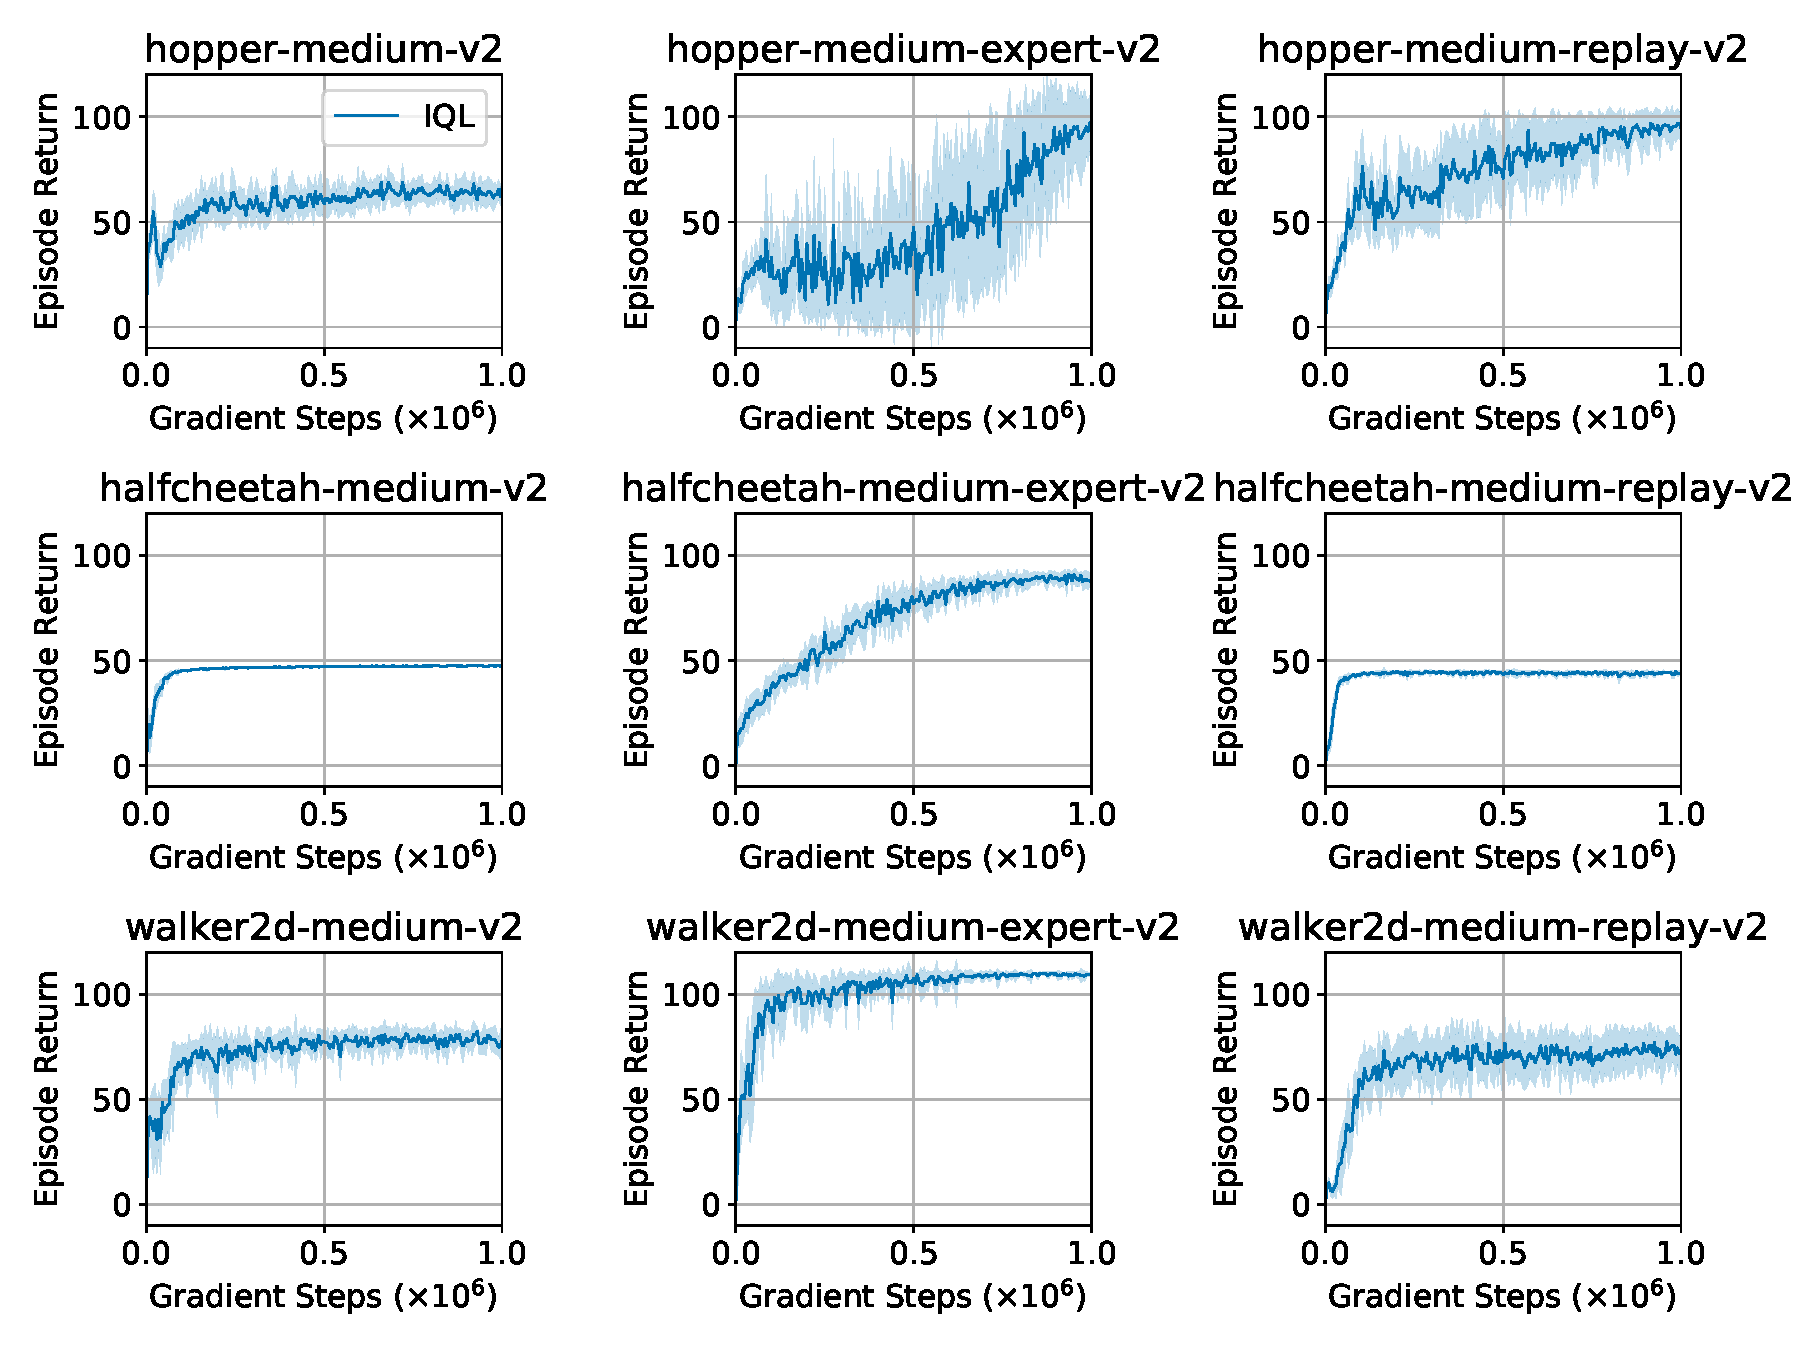
\includegraphics[width=\textwidth]{images/curves_mujoco.pdf}
    \caption{Learning curves for MuJoCo locomotion tasks.}
    \label{fig:curves_mujoco}
\end{figure}

\begin{figure}
    \centering
    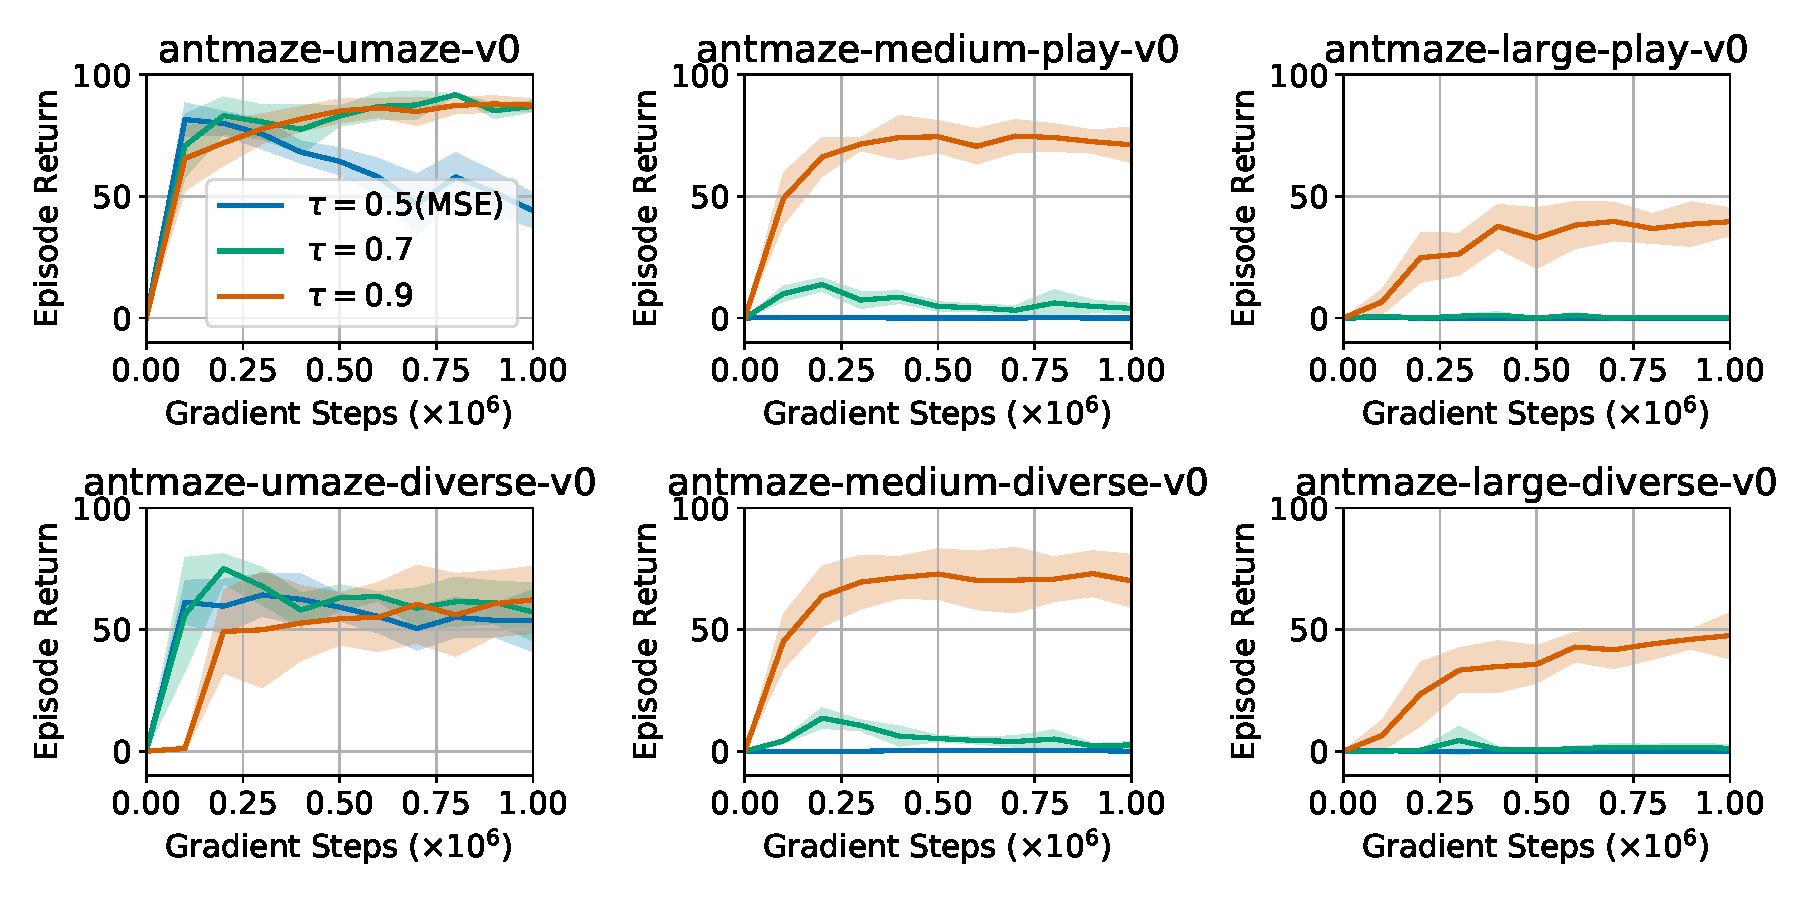
\includegraphics[width=\textwidth]{images/antmaze_full.pdf}
    \caption{Results on Ant Maze for different values of $\tau$. Note that $\tau=0.5$ corresponds to using the mean squared error instead of expectile regression.}
    \label{fig:antmaze_full}
\end{figure}

\begin{table}[b]\centering
\caption{Effect of $\tau$. Fitting $V(s)$ with mean squared error ($\tau=0.5$) is not sufficient to propagate the signal through recursion and fails to solve more challenging medium and large tasks.}\label{tab:antmaze-full}
\scriptsize
\begin{tabular}{l||rrrr}
&IQL w/ $\tau=0.5$ (MSE) &IQL w/ $\tau=0.7$ &IQL w/ $\tau=0.9$ \\\hline
antmaze-umaze-v0 &44.2$\pm$7.2 &87.0$\pm$2.3 &87.5$\pm$2.6 \\
antmaze-umaze-diverse-v0 &53.6 $\pm$12.7 &57.2$\pm$11.9 &62.2$\pm$13.8 \\
antmaze-medium-play-v0 &0.0$\pm$0.0 &4.0$\pm$2.0 &71.2 $\pm$7.3 \\
antmaze-medium-diverse-v0 &0.0 $\pm$0.0 &2.6$\pm$1.4 &70.0$\pm$10.9 \\
antmaze-large-play-v0 &0.0$\pm$0.0 &0.2$\pm$0.4 &39.6 $\pm$5.8 \\
antmaze-large-diverse-v0 &0.0 $\pm$0.0 &1.2$\pm$1.6 &47.5$\pm$9.5 \\ \hline \hline
total &97.8$\pm$19.9 &152.2$\pm$19.6 &378.0$\pm$49.9 \\
\end{tabular}
\end{table}

\paragraph{Results on Franca Kitchen and Adoit tasks.}
For Franca Kitchen and Adroit tasks we use $\tau=0.7$ and the inverse temperature $\beta=0.5$. Due to the size of the dataset, we also apply Dropout~\citep{srivastava2014dropout} with dropout rate of $0.1$ to regularize the policy network. See complete results in \Cref{tab:franca_adroit}.


\begin{table}[!htp]\centering
\caption{Evaluation on Franca Kitchen and Adroit tasks from D4RL}\label{tab:franca_adroit}
\scriptsize
\begin{tabular}{l||rrrrr|r}
dataset &BC &BRAC-p &BEAR &Onestep RL &CQL &Ours \\ \hline
kitchen-complete-v0 &\textbf{65.0} &0.0 &0.0 &- &43.8 &\textbf{62.5} \\
kitchen-partial-v0 &38.0 &0.0 &0.0 &- &\textbf{49.8} &\textbf{46.3} \\
kitchen-mixed-v0 &\textbf{51.5} &0.0 &0.0 &- &\textbf{51.0} &\textbf{51.0} \\ \hline
kitchen-v0 total &\textbf{154.5} &0.0 &0.0 &- &144.6 &\textbf{159.8} \\ \hline
pen-human-v0 &63.9 &8.1 &-1.0 &- &37.5 &\textbf{71.5} \\
hammer-human-v0 &1.2 &0.3 &0.3 &- &\textbf{4.4} &1.4 \\
door-human-v0 &2 &-0.3 &-0.3 &- &\textbf{9.9} &4.3 \\
relocate-human-v0 &0.1 &-0.3 &-0.3 &- &0.2 &0.1 \\
pen-cloned-v0 &37 &1.6 &26.5 &\textbf{60.0} &39.2 &37.3 \\
hammer-cloned-v0 &0.6 &0.3 &0.3 &\textbf{2.1} &\textbf{2.1} &\textbf{2.1} \\
door-cloned-v0 &0.0 &-0.1 &-0.1 &0.4 &0.4 &\textbf{1.6} \\
relocate-cloned-v0 &-0.3 &-0.3 &-0.3 &-0.1 &-0.1 &-0.2 \\ \hline
adroit-v0 total &104.5 &9.3 &25.1 &- &93.6 &\textbf{118.1} \\ \hline \hline
total &259 &9.3 &25.1 &- &238.2 &\textbf{277.9} \\
\end{tabular}
\end{table}

\section{Finetuning experimental details}
\label{app:finetuning}
For finetuning experiments, we first run offline RL for 1M gradient steps. Then we continue training while collecting data actively in the environment and adding that data to the replay buffer, running 1 gradient update / environment step. All other training details are kept the same between the offline RL phase and the online RL phase. For dextrous manipulation environments~\citep{rajeswaran2018dextrous}, we use $\tau=0.8$ and $\beta=3.0$, 25000 offline training steps, and add Gaussian noise with standard deviation $\sigma=0.03$ to the policy for exploration.

\begin{wraptable}[12]{r}{0.55\textwidth}
% \begin{table}[!htp]\centering
\scriptsize
\begin{tabular}{ l ||p{1.5cm} | p{1.5cm}  }
    \centering
    Dataset & Offline & Online \\
    % Dataset & AWAC \; Offline$\rightarrow$Online & CQL Offline $\rightarrow$ Online & Ours Offline $\rightarrow$ Online \\
    \hline
    antmaze-umaze-v0 & 70.1 \; $\rightarrow$ \textbf{99.4} & \textbf{86.7} \; $\rightarrow$ \textbf{96.0} \\
    antmaze-umaze-diverse-v0 & 31.1 \; $\rightarrow$ \textbf{99.4} & \textbf{75.0} \; $\rightarrow$ 84.0 \\
    antmaze-medium-play-v0 & 23.0 \; $\rightarrow$ 0.0 & \textbf{72.0} \; $\rightarrow$ \textbf{95.0} \\
    antmaze-medium-diverse-v0 & 23.0 \; $\rightarrow$ 32.3 & \textbf{68.3} \; $\rightarrow$ \textbf{92.0} \\
    antmaze-large-play-v0 & 1.0 \; \; $\rightarrow$ 0.0 & \textbf{25.5} \; $\rightarrow$ \textbf{46.0} \\
    antmaze-large-diverse-v0 & 1.0 \; \; $\rightarrow$ 0.0 & \textbf{42.6} \; $\rightarrow$ \textbf{60.7} \\ \hline
    % antmaze-v0 total & 151.5 $\rightarrow$ 231.1 & \textbf{370.1} $\rightarrow$ \textbf{473.7} \\ \hline
    pen-binary-v0 & 46.2 $\pm$ 6.3 & 63.3 \; $\pm$ 1.9 \\
    door-binary-v0 & 1.3 \; $\pm$ 0.7 & 42.0 \; $\pm$ 3.2 \\
    relocate-binary-v0 & 0.3 \; $\pm$ 0.4 & 23.3 \; $\pm$ 14.5 \\ \hline
    % hand-v0 total & 31.5 \; $\rightarrow$ 9.9 & 38.1 \; $\rightarrow$ \textbf{124.0} \\ \hline \hline
    % total & 182.8 $\rightarrow$ 241.0 & \textbf{408.2} $\rightarrow$ \textbf{597.7}
    %%SL.10.3: why is CQL offline ant maze much worse here than it is in Table 1? is that a bug?
\end{tabular}
\caption{Error bars for fine-tuning experiments with 20 seeds, showing one standard deviation.}
\label{tab:finetuning}
% \end{table}
\end{wraptable}

For baselines we compare to the original implementations of AWAC~\citep{nair2020awac} and CQL~\citep{kumar2020conservative}. For AWAC we used \url{https://github.com/rail-berkeley/rlkit/tree/master/rlkit}. We found AWAC to overfit heavily with too many offline gradient steps, and instead used 25000 offline gradient steps as in the original paper. For the dextrous manipulation results, we report average return normalized from 0 to 100 for consistency, instead of success rate at the final timestep, as reported in~\citet{nair2020awac}. For CQL, we used \url{https://github.com/aviralkumar2907/CQL}. Our reproduced results offline are worse than the reported results, particularly on medium and large antmaze environments. We were not able to improve these results after checking for discrepancies with the CQL paper authors and running CQL with an alternative implementation (\url{https://github.com/tensorflow/agents}). Thus, although for offline experiments (Table~\ref{tab:d4rl}) we report results from the original paper, for finetuning experiments we did not have this option and report our own results running CQL in Table~\ref{tab:finetuning}.

\section{Connections to prior work}
In this section, we discuss how our approach is related to prior work on offline reinforcement learning. In particular, we discuss connections to BCQ~\cite{fujimoto2019off}.
%, Onestep RL~\cite{brandfonbrener2021offline} and AWAC~\cite{nair2020awac}.

Our batch constrained optimization objective is similar to BCQ~\citep{fujimoto2019off}. In particular, the authors of BCQ build on the Q-learning framework and define the policy as
\begin{equation}
\label{eqn:bcq_policy}
\pi(s) = \argmax_{\substack{a\\s.t.(s, a)\in \D}}Q(s,a).
\end{equation}
Note that in contrast to the standard Q-learning, maximization in \Cref{eqn:bcq_policy} is performed only over the state-action pairs that appear in the dataset. In \cite{fujimoto2019off}, these constraints are implemented via fitting a generative model $\mu(\cdot|s)$ on the dataset, sampling several candidate actions from this generative model, and taking an argmax over these actions:
$$
\pi(s) = \argmax_{\{a_i| a_i \sim \mu(\cdot|s), i=1\ldots N\}}Q(s,a_i).
$$
However, this generative model can still produce out-of-dataset actions that will lead to querying undefined Q-values. Thus, our work introduces an alternative way to optimize this objective without requiring an additional density model. Our approach avoids this issue by enforcing the hard constraints via estimating expectiles. Also, it is worth mentioning that a number of sampled actions $N$ in BCQ has similar properties to choosing a particular expectile $\tau$ in our approach.


Note that our algorithm for optimal value approximation does not require an explicit policy, in contrast to other algorithms for offline reinforcement learning for continuous action spaces~\citep{fujimoto2019off, fujimoto2021minimalist, wu2019behavior, kostrikov2021offline, kumar2019stabilizing, kumar2020conservative}. Thus, we do not need to alternate between actor and critic updates, though with continuous actions, we must still extract an actor at the end once the critic converges.

\section{Different Estimators of $V(s)$}

{
We also evaluate different ways to estimate the value function $V(s)$ (\Cref{tab:abm}). We compare $V(s)$ learned with expectile regression as in IQL with $V(s)$ estimated with several samples from the learned policy as in ABM~\citep{siegel2020keep}. In particular, we use $N=20$ to estimate the value function.}


\begin{table}[!htp]\centering
\caption{Different estimators of $V(s)$}\label{tab:abm}
\scriptsize
\begin{tabular}{l|rrr}
&IQL & $V(s)=\sum_{i=1}^N Q(s,a_i) / N$ \\\hline
hopper-medium-v2 &66.2$\pm$5.7 &69.5$\pm$3.9 \\
hopper-medium-expert-v2 &91.5$\pm$14.3 &75.8$\pm$37.8 \\
hopper-medium-replay-v2 &94.7$\pm$8.6 &64.7$\pm$22.6 \\
halfcheetah-medium-v2 &47.4$\pm$0.2 &47.2$\pm$0.2 \\
halfcheetah-medium-expert-v2 &86.7$\pm$5.3 &93.0$\pm$0.9 \\
halfcheetah-medium-replay-v2 &44.2$\pm$1.2 &45.1$\pm$0.3 \\
walker2d-medium-v2 &78.3$\pm$8.7 &72.0$\pm$24.6 \\
walker2d-medium-expert-v2 &109.6$\pm$1.0 &110.7$\pm$0.4 \\
walker2d-medium-replay-v2 &73.8$\pm$7.1 &83.3$\pm$3.0 \\ \hline
locomotion total &692.4$\pm$52.1 &661.4$\pm$93.7 \\ \hline
antmaze-umaze-v0 &87.5$\pm$2.6 &96.4$\pm$1.8 \\
antmaze-medium-play-v0 &71.2$\pm$7.3 &0.0$\pm$0.0 \\
antmaze-large-play-v0 &39.6$\pm$5.8 &0.0$\pm$0.0 \\
antmaze-umaze-diverse-v0 &62.2$\pm$13.8 &57.5$\pm$6.3 \\
antmaze-medium-diverse-v0 &70.0$\pm$10.9 &0.0$\pm$0.0 \\
antmaze-large-diverse-v0 &47.5$\pm$9.5 &0.0$\pm$0.0 \\ \hline
antmaze total &378.0$\pm$49.9 &153.9$\pm$8.1 \\
\end{tabular}
\end{table}
\end{document}
